%
% this file is encoded in utf-8
% v1.7

\documentclass[12pt, a4paper]{ntust_report}




% 除非校方修改了論文格式 (margins, header, footer, 浮水印)
% 或者需要增加所用的 LaTeX 套件,
% 或者要改預設中文字型、編碼
% 否則毋須修改本檔內容
% 論文撰寫,請修改以 my_  開頭檔名的各檔案

\usepackage{CJK}  %%% ZZZ %%% macro for Chinese/Japanese/Korean processing
\usepackage[nospace]{cite}  % for smart citation
\usepackage{geometry}  % for easy margin settings
\usepackage{subfigure}  % for subfigure
%
% margins setting
\geometry{verbose,a4paper,tmargin=3.5cm,bmargin=2cm,lmargin=3cm,rmargin=3cm}
%
\usepackage{amsmath} % 各式 AMS 數學功能
\usepackage{amssymb} % 各式 AMS 數學符號
\usepackage{mathrsfs} %草寫體數學符號,在數學模式裡用 \mathscr{E} 得草寫 E
\usepackage{listings} % 程式列表套件
%
% listing setting
\lstset{breaklines=true,% 過長的程式行可斷行
extendedchars=false,% 中文處理不需要 extendedchars
texcl=true,% 中文註解需要有 TeX 處理過的 comment line, 所以設成 true
comment=[l]\%\%,% 以雙「百分號」做為程式中文註解的起頭標記,配合 MATLAB
basicstyle=\small,% 小號字體, 約 10 pt 大小
commentstyle=\upshape,% 預設是斜體字,會影響註解裏的英文,改用正體
%language=Octave % 會將一些 octave 指令以粗體顯示
}

\usepackage{url} % 在文稿中引用網址,可以用 \url{http://www.ntust.edu.tw} 方式

% 插圖套件 graphicx
% 使用者工作流程是用 pdftex 還是 latex + dvipdfmx?
% 視情況而有不同的參數
% 這裡作自動判斷
% 參考自
% http://www.tex.ac.uk/cgi-bin/texfaq2html?label=ifpdf

\ifx\pdfoutput\undefined
  % not running pdftex
  \usepackage[dvipdfm]{graphicx}
\else
  \ifx\pdfoutput\relax
    % not running pdftex
    \usepackage[dvipdfm]{graphicx}
  \else
    % running pdftex, with...
    \ifnum\pdfoutput>0
      % ... PDF output
      \usepackage[pdftex]{graphicx}
    \else
      %...DVI output
      \usepackage[dvipdfm]{graphicx}
    \fi
  \fi
\fi

\usepackage{fancyhdr}  % 借用增強功能型 header 套件來擺放浮水印 
% (佔用了 central header)
% 不需要浮水印的使用者仍可利用此套件,產生所需的 header, footer
%
% 啟動 fancy header/footer 套件
\pagestyle{fancy}
\fancyhead{}  % reset left, central, right header to empty
\fancyfoot[C]{\thepage} %中間 footer 擺放頁碼
\renewcommand{\headrulewidth}{0pt} % header 的直線; 0pt 則無線

% 如果不需要任何浮水印,則請把下列介於 >>> 與 <<< 之間
% 的文字行關掉 (行首加上百分號)
%% 浮水印 >>> 
%
% this file is encoded in utf-8
% v1.7
% 如果浮水印不是全篇需要,請把下列介於 >>> 與 <<<
% 的「全篇浮水印專用碼」關掉 (行首加百分號)
% 參考自 Keith Reckdahl 寫的 "Using Imported Graphics in LATEX2e" (epslatex.pdf) p.39
% 如果只有特定頁需要浮水印
% 則依該頁屬性使用下列之一的命令 
% 普通頁命令 \thispagestyle{WaterMarkPage}
% plain 頁命令 \thispagestyle{PlainWaterMarkPage}
% empty 頁命令 \thispagestyle{EmptyWaterMarkPage}


% 將重複使用的浮水印章
% 圖檔是 my_watermark.xxx
% 副檔名可以不加,可以是 latex 系統能處裡的任何格式:pdf, gif, png, jpg, eps, ...
% 某些圖檔格式在某些工作流程可能需要作前置處裡。
% 例如,pdflatex 無法直接處理 eps 檔
%  latex + dvipdfmx 無法直接處理 pdf, gif, png, jpg, 需要用 ebb 小工具程式
%  對圖檔產生 .bb 對應檔。
% old code
%\newsavebox{\mywatermark}
%\sbox{\mywatermark}{\includegraphics[keepaspectratio,%
%height=0.8\textheight,%
%width=0.8\textwidth]{my_watermark}}
% new code
\newsavebox{\mywatermark}
\sbox{\mywatermark}{
\includegraphics[keepaspectratio,%
width=2.5cm]{watermark/ntust_watermark}}


% 將 central header 擺放浮水印的巨集指令
\newcommand{\PlaceWaterMark}{\fancyhead[C]{\setlength{\unitlength}{1in}%
\begin{picture}(0,0)%
%\put(-2.2,-6){\usebox{\mywatermark}}% old code
\put(-0.5,-6.2){\usebox{\mywatermark}}% new code
\end{picture}}%
}

\fancyhead{}  % reset left, central, right header to empty
%% 如果不需整篇論文都要浮水印
%% 則下面  >>> 與 <<< 之間的程式碼請關閉
%% >>> 全篇浮水印
\PlaceWaterMark  % 每一頁都有浮水印 (除了 plain、empty 頁以外)

% 重新定義 plain 頁面
% 每張 plain 頁面 (每一章的第一頁) 也加浮水印

\fancypagestyle{plain}{%
\fancyhead{}%
\PlaceWaterMark%
\fancyfoot{}%
\fancyfoot[C]{\thepage}
\renewcommand{\headrulewidth}{0pt}%
\renewcommand{\footrulewidth}{0pt}%
}
%% <<< 全篇浮水印

%% 如果只有一、兩頁需要有浮水印
%% 可以在該頁 (有頁碼) 使用 \thispagestyle{WaterMarkPage}
%% 此命令不影響原有的 header、footer
\fancypagestyle{WaterMarkPage}{%
\PlaceWaterMark%
}

%% 如果只有一、兩頁 plain 頁需要有浮水印 (如 摘要、自傳等)
%% 可以在該頁 (有頁碼) 使用 \thispagestyle{PlainWaterMarkPage}
%% 只有頁碼與浮水印,沒有其他的 header、footer
%% 等同於 plain page style + water mark
\fancypagestyle{PlainWaterMarkPage}{%
\fancyhead{}%
\PlaceWaterMark%
\fancyfoot{}%
\fancyfoot[C]{\thepage}
\renewcommand{\headrulewidth}{0pt}%
\renewcommand{\footrulewidth}{0pt}%
}

%% 如果只有一、兩頁 empty 頁需要有浮水印 (如封面、書名頁)
%% 可以在該頁 (無頁碼) 使用 \thispagestyle{EmptyWaterMarkPage}
%% 等同於 empty page style + water mark
\fancypagestyle{EmptyWaterMarkPage}{%
\fancyhead{}%
\PlaceWaterMark%
\fancyfoot{}%
\renewcommand{\headrulewidth}{0pt}%
\renewcommand{\footrulewidth}{0pt}%
}

%% <<< 浮水印



% global page layout
\newcommand{\mybaselinestretch}{1.5}  %行距 1.5 倍 + 20%, (約為 double space)
\renewcommand{\baselinestretch}{\mybaselinestretch}  % 論文行距預設值
\parskip=2ex  % 段落之間的間隔為兩個 x 的高度
\parindent = 0Pt  % 段首內縮由 CJK 控制,所以這裡就設成不內縮

%%%%%%%%%%%%%%%%%%%%%%%%%%%%%
%  end of preamble
%%%%%%%%%%%%%%%%%%%%%%%%%%%%%  %基本的環境設定  無需改變  
\usepackage{amsmath}
\usepackage{cite}     % Sort all citations
\usepackage{psfrag}   % Used to insert text into figures
\usepackage{graphicx}
\usepackage{xspace}
\usepackage{subfigure}
\usepackage{url}
\usepackage{hyperref}
\usepackage{indentfirst}
\usepackage{color}
\def\blue{\color{blue}}
\def\red{\color{red}}
\def\orange{\color{orange}}
% \usepackage{cite}     % Sort all citations


%\usepackage{subcaption}
%%%--------------------%%
\usepackage{float}
%\usepackage{amssymb}
%\usepackage{amsfonts}
%\usepackage{epstopdf}
%\usepackage{algpseudocode}
%\usepackage{caption}
%\captionsetup{compatibility=false}
%\usepackage{xspace}
%%%---------------------%%

\usepackage{algorithmic} % pseudocode
\usepackage{algorithm}
\usepackage{float}
\usepackage{amssymb}
\floatname{algorithm}{Method}

\usepackage{xspace}


\def\centerhack#1{\hbox to 0pt{\hss\footnotesize #1\hss}}
\def\dchack#1{\vbox to 0pt{\vss{\hbox to 0pt{\hss#1\hss}}\vss}}

\newcounter{linecounter}
\newcommand{\resetlinecounter}{\setcounter{linecounter}{1}}
\newcommand{\llabel}[1]{\arabic{linecounter}. \addtocounter{linecounter}{-1}\refstepcounter{linecounter}\label{#1}\stepcounter{linecounter}}
\newcommand{\declabel}{\addtocounter{linecounter}{-1}}

\newcommand{\aboveleftarrow}[1]{{\buildrel #1 \over \longleftarrow}}
\newcommand{\aboverightarrow}[1]{{\buildrel #1 \over \longrightarrow}}
\newcommand{\aboveleftrightarrow}[1]{{\buildrel #1 \over
    \leftrightarrow}}

\renewcommand{\paragraph}[1]{\vspace{2mm}\noindent{\textbf{#1}}\quad}

\newcommand{\sign}[2]{\textrm{Sign}_{#2}(#1)}
\newcommand{\signature}[2]{\sigma_{#2}(#1)}

\newtheorem{theorem}{Theorem}[section]
\newtheorem{conjecture}[theorem]{Conjecture}
\newtheorem{corollary}[theorem]{Corollary}
\newtheorem{proposition}[theorem]{Proposition}
\newtheorem{lemma}[theorem]{Lemma}

%\hfuzz=\maxdimen
%\tolerance=10000
%\hbadness=10000

\begin{document}
\begin{CJK}{UTF8}{bsmi}   %%% ZZZ %%%  <<< 在這裡更改預設中文字型、編碼
% 編碼:UTF8, Bg5, ...
% 中文字型名稱:TeXLive 安裝有一套明體字 bsmi, 楷書與其他字型視你的 LaTeX CJK 系統裝設情況而定
% 注意! 修改時請一併修改此檔案末端之\end{ZZZ}
% global CJK setting
\CJKindent  %%% ZZZ %%%  段首內縮兩格

% 下列中文名詞的定義,如果以註解方式關閉取消,
% 則會以系統原先的預設值 (英文) 替代
% 名詞 \prechaptername 預設值為 Chapter
% 名詞 \postchaptername 預設值為空字串
% 名詞 \tablename 預設值為 Table
% 名詞 \figurename 預設值為 Figure
\renewcommand\prechaptername{\textit{Chapter}} % 出現在每一章的開頭的「第 x 章」
\renewcommand\postchaptername{\\}
\renewcommand{\tablename}{Table} % 在文章中 table caption 會以「表 x」表示
\renewcommand{\figurename}{Figure} % 在文章中 figure caption 會以「圖 x」表示

% 下列中文名詞的定義,用於論文固定的各部分之命名 (出現於目錄與該頁標題)
\newcommand{\nameInnerCover}{教授推薦書}
\newcommand{\nameCommitteeForm}{論文口試委員審定書}
\newcommand{\nameCopyrightForm}{授權書}
%\newcommand{\nameCabstract}{中文摘要}
\newcommand{\nameEabstract}{Abstract}
\newcommand{\nameAckn}{Acknowledgment}
\newcommand{\nameToc}{Table of contents}
\newcommand{\nameLot}{List of Tables}
\newcommand{\nameTof}{List of Figures}
%\newcommand{\nameSlist}{符號說明}
\newcommand{\nameRef}{References}
%\newcommand{\nameVita}{自傳}
 %在此檔案處定義文章中的中文名詞

	%---------------------------------------------------------------------------------

	%
% this file is encoded in utf-8
% v1.7
% do not change the content of this file
% unless the thesis layout rule is changed
% 無須修改本檔內容,除非校方修改了
% 封面、書名頁、中文摘要、英文摘要、誌謝、目錄、表目錄、圖目錄、符號說明
% 等頁之格式
% this file is encoded in utf-8
%v1.7

% make the line spacing in effect
\renewcommand{\baselinestretch}{\mybaselinestretch}
\large % it needs a font size changing command to be effective
 
 \newcommand\cTitle{}
\newcommand\eTitle{}
\newcommand\myCname{}
\newcommand\myEname{}
\newcommand\myStudentID{}
\newcommand\advisorCnameA{}
\newcommand\advisorEnameA{}
\newcommand\advisorCnameB{}
\newcommand\advisorEnameB{}
\newcommand\advisorCnameC{}
\newcommand\advisorEnameC{}
\newcommand\univCname{}
\newcommand\univEname{}
\newcommand\deptCname{}
\newcommand\fulldeptEname{}
\newcommand\deptEname{}
\newcommand\collEname{}
\newcommand\degreeCname{}
\newcommand\degreeEname{}
\newcommand\cYear{}
\newcommand\cMonth{}
\newcommand\cDay{}
%\newcounter{eYear}
\newcommand\eYear{}
\newcommand\eMonth{}
\newcommand\ePlace{}

%
% this file is encoded in utf-8
% v1.7
% 填入你的論文題目、姓名等資料
% 如果題目內有必須以數學模式表示的符號,請用 \mbox{} 包住數學模式,如下範例
% 如果中文名字是單名,與姓氏之間建議以全形空白填入,如下範例
% 英文名字中的稱謂,如 Prof. 以及 Dr.,其句點之後請以不斷行空白~代替一般空白,如下範例
% 如果你的指導教授沒有如預設的三位這麼多,則請把相對應的多餘教授的中文、英文名
%    的定義以空的大括號表示
%    如,\renewcommand\advisorCnameB{}
%          \renewcommand\advisorEnameB{}
%          \renewcommand\advisorCnameC{}
%          \renewcommand\advisorEnameC{}

% 論文題目 (中文)
\renewcommand\cTitle{
在第一人稱視角下使用時間聚合技術做動作辨識
}

% 論文題目 (英文)
\renewcommand\eTitle{%My Thesis Title  
Temporal Aggregation for Action Recognition in First-Person Video
}

% 我的姓名 (中文)
\renewcommand\myCname{}

% 我的姓名 (英文)
\renewcommand\myEname{Didik~Purwanto}

%我的學號
\renewcommand\myStudentID{M10402804}
% 指導教授A的姓名 (中文)
\renewcommand\advisorCnameA{}

% 指導教授A的姓名 (英文)
\renewcommand\advisorEnameA{Professor Wen-Hsien Fang}

% 指導教授B的姓名 (中文)
\renewcommand\advisorCnameB{}

% 指導教授B的姓名 (英文)
\renewcommand\advisorEnameB{Professor Yie-Tarng Chen}
% 指導教授C的姓名 (中文)
\renewcommand\advisorCnameC{}

% 指導教授C的姓名 (英文)
\renewcommand\advisorEnameC{}

% 校名 (中文)
\renewcommand\univCname{國立台灣科技大學}

% 校名 (英文)
%\renewcommand\univEname{National Taiwan University of science and technology}

% 系所名 (中文)
\renewcommand\deptCname{電~子~工~程~系}

% 系所全名 (英文)
%\renewcommand\fulldeptEname{Graduate School of Electro-Optical Engineering}

% 系所短名 (英文, 用於書名頁學位名領域)
%\renewcommand\deptEname{Electro-Optical Engineering}

% 學院英文名 (如無,則以空的大括號表示)
%\renewcommand\collEname{College of Electrical and Communication Engineering}

% 學位名 (中文)
\renewcommand\degreeCname{碩士}

% 學位名 (英文)
%\renewcommand\degreeEname{Master of Science}

% 口試年份 (中文、民國)
\renewcommand\cYear{ 106 }

% 口試月份 (中文)
\renewcommand\cMonth{ 7 } 

% 口試月份 (中文)
\renewcommand\cDay{ 23 } 


% 學校所在地 (英文)
\renewcommand\ePlace{Taipei, Taiwan}

%畢業級別;用於書背列印;若無此需要可忽略
\newcommand\GraduationClass{}

%%%%%%%%%%%%%%%%%%%%%%


\newcommand\itsempty{}


%%%%%%%%%%%%%%%%%%%%%%%%%%%%%%%
%       ntust cover 封面
%%%%%%%%%%%%%%%%%%%%%%%%%%%%%%%


\begin{titlepage}
% no page number
% next page will be page 1

% aligned to the center of the page
\begin{center}

\begin{figure}[htbp]
	\begin{minipage}[b]{5cm} 
	\raggedright
	
\includegraphics[width=1in]{figures/ntust_logo.jpg}
	\label{fig:ntust_logo}
	\end{minipage}% 
	\begin{minipage}[b]{0.5\textwidth} 
	\centering
	\makebox[3cm][c]{\Huge{\univCname}}\\  %顯示中文校名
	\vspace{0.5cm}
	\makebox[3cm][c]{\Huge{\deptCname}}\\ %顯示中文系所名
	\vspace{0.5cm}
	\end{minipage}%
\\ 
\rule{16cm}{3pt}
\end{figure}
\hfill


\vspace{2.5cm}
\makebox[6cm][s]{\textbf{\Huge{\degreeCname 學位論文 }}}\\ %顯示論文種類 (中文)
\vspace{2.5cm}
%
% Set the line spacing to single for the titles (to compress the lines)
\renewcommand{\baselinestretch}{1}   %行距 1 倍
%\large % it needs a font size changing command to be effective
\Large{\cTitle}\\  % 中文題目
%
\vspace{1cm}
%
\Large{\eTitle}\\ %英文題目
\vspace{1cm}
% \makebox is a text box with specified width;
% option s: stretch
% use \makebox to make sure
% 「研究生:」 與「指導教授:」occupy the same width
\vspace{1cm} 
\Large{\myEname}  % 顯示作者中文名

\vspace{0.5cm} 
\Large{\myStudentID}  %顯示指導教授A中文名

\vspace{1cm}
%

 \hspace{1cm}\makebox[3cm][s]{\Large{指導教授:}}
\Large{\advisorEnameA}  %顯示指導教授A中文名
 \makebox[1cm][s]{}\\
%
% 判斷是否有共同指導的教授 B
\ifx \advisorEnameB  \itsempty
\relax % 沒有 B 教授,所以不佔版面,不印任何空白
\else
% 共同指導的教授 B
\hspace{4.5cm} \makebox[0.95 cm][s]{}
\Large{\advisorEnameB}  %顯示指導教授B中文名
\hfill \makebox[2cm][s]{}\\
\fi
%
% 判斷是否有共同指導的教授 C
\ifx \advisorCnameC  \itsempty
\relax % 沒有 C 教授,所以不佔版面,不印任何空白
\else
% 共同指導的教授 C
\hspace{4.5cm} \makebox[3cm][s]{}
\Large{\advisorCnameC}  %顯示指導教授C中文名
\hfill \makebox[1cm][s]{}\\
\fi
%
\vfill
\makebox[10cm][s]{\Large{中華民國\cYear 年\cMonth 月\cDay 日}}%
%
\\




\end{center}
% Resume the line spacing to the desired setting
\renewcommand{\baselinestretch}{\mybaselinestretch}   %恢復原設定
% it needs a font size changing command to be effective
% restore the font size to normal
\normalsize
\end{titlepage}

%%%%%%%%%%%%%%%

%% 從摘要到本文之前的部份以小寫羅馬數字印頁碼
% 但是從「書名頁」(但不印頁碼) 就開始計算
\setcounter{page}{1}
\pagenumbering{roman}
%%%%%%%%%%%%%%%%%%%%%%%%%%%%%%%
%       指導教授推薦書 
%%%%%%%%%%%%%%%%%%%%%%%%%%%%%%%
%

% insert the printed standard form when the thesis is ready to bind
% 在口試完成後,再將已簽名的推薦書放入以便裝訂
% create an entry in table of contents for 推薦書
% 目前送出空白頁

%\newpage{\thispagestyle{empty}\addcontentsline{toc}{chapter}{\nameInnerCover}\mbox{}\clearpage}
%\newpage

%教授推薦書\newgeometry{tmargin=0.1cm,bmargin=0.1cm,lmargin=1cm,rmargin=0.1cm}
%\begin{flushleft}
%\includegraphics[width=\textwidth]{frontpages/thesis_form1.jpeg}
%\end{flushleft}



% 判斷是否要浮水印?
\ifx\mywatermark\undefined 
  \thispagestyle{empty}  % 無頁碼、無 header (無浮水印)
\else
  \thispagestyle{EmptyWaterMarkPage} % 無頁碼、有浮水印
\fi



%%%%%%%%%%%%%%%%%%%%%%%%%%%%%%%%
%%       英文摘要 
%%%%%%%%%%%%%%%%%%%%%%%%%%%%%%%%
%
\newpage
\thispagestyle{plain}  % 無 header,但在浮水印模式下會有浮水印

% create an entry in table of contents for 英文摘要
\addcontentsline{toc}{chapter}{\nameEabstract}

% aligned to the center of the page
\begin{center}
% font size:
% \large (14pt) < \Large (18pt) < \LARGE (20pt) < \huge (24pt)< \Huge (24 pt)
% Set the line spacing to single for the names (to compress the lines)
\renewcommand{\baselinestretch}{1}   %行距 1 倍
%\large % it needs a font size changing command to be effective
%\large{\eTitle}\\  %英文題目
%\vspace{0.83cm}
% \makebox is a text box with specified width;
% option s: stretch
% use \makebox to make sure
% each text field occupies the same width
%\makebox[2cm][s]{\large{Student: }}
%\makebox[5cm][l]{\large{\myEname}} %學生英文姓名
%\hfill
%
%\makebox[2cm][s]{\large{Advisor: }}
%\makebox[5cm][l]{\large{\advisorEnameA}} \\ %教授A英文姓名
%
% 判斷是否有共同指導的教授 B
\ifx \advisorCnameB  \itsempty
\relax % 沒有 B 教授,所以不佔版面,不印任何空白
\else
%共同指導的教授B
\makebox[2cm][s]{}
\makebox[5cm][l]{} %%%%%
\hfill
\makebox[2cm][s]{}
\makebox[5cm][l]{\large{\advisorEnameB}}\\ %教授B英文姓名
\fi
%
% 判斷是否有共同指導的教授 C
\ifx \advisorCnameC  \itsempty
\relax % 沒有 C 教授,所以不佔版面,不印任何空白
\else
%共同指導的教授C
\makebox[2cm][s]{}
\makebox[5cm][l]{} %%%%%
\hfill
\makebox[2cm][s]{}
\makebox[5cm][l]{\large{\advisorEnameC}}\\ %教授C英文姓名
\fi
%
%\vspace{0.42cm}
%\large{Submitted to }\large{\fulldeptEname}\\  %英文系所全名
%
%\ifx \collEname  \itsempty
%\relax % 如果沒有學院名 (英文),則不佔版面,不印任何空白
%\else
% 有學院名 (英文)
%\large{\collEname}\\% 學院名 (英文)
%\fi
%
%\large{\univEname}\\  %英文校名
%\vspace{0.83cm}
%\vfill
%
\large{\textbf{Abstract}}\\
\vspace{0.5cm}
\end{center}
% Resume the line spacing the desired setting
\renewcommand{\baselinestretch}{\mybaselinestretch}   %恢復原設定
%\large %it needs a font size changing command to be effective
% restore the font size to normal
\normalsize
%%%%%%%%%%%%%


\blue{
First person point of view video is a video produced by 
egocentic camera that capture the scene with first person perspective. 
The characteristic of the first-person point of view video 
in general features are rich in noise and contain plenty of uncontrolled variations scene.
Moreover, these videos need to deal with some adverse effects such as shaky frame, background clutter, occlusion and inter-class variation. Coupled with the absence of the actor's pose, 
it makes the first-person video is more challenging than the third person video.
}

This \blue{thesis} presents a new approach for action recognition in
first-person videos which aggregates both of the short- and
long-term trends based on the coefficients of the Hilbert-Huang
transform (HHT), a renowned time-frequency analysis tool. In
contrast to previous works like Pooled Time Series (PoT), the new
approach can extract the salient features of activities based on the
non-stationary HHT analysis, which consists of empirical mode
decomposition and Hilbert spectral analysis. The proposed approach
can be incorporated with the convolutional neural network (CNN)
features such as trajectory pooled CNN features to
achieve superior detection accuracy. Simulations show that
the proposed method outperforms the main state-of-the-art works on
\blue{three} widespread public first-person datasets.

\textbf{Keywords}: temporal pyramid pooling, temporal
aggregation, first-person video, action recognition, Hilbert-Huang transform


%%%%%%%%%%%%%%%%%%%%%%%%%%%%%%%%
%%       Publications
%%%%%%%%%%%%%%%%%%%%%%%%%%%%%%%%


\newpage
\chapter*{\protect\makebox[5cm][s]{Related Publications}} 
\addcontentsline{toc}{chapter}{Related Publications}


%\textbf{Journal}
%\begin{itemize}
%    \item  \textbf{Didik Purwanto}, Yie-Tarng Chen, Wen-Hsien Fang, Erick Hendra Putra Alwando, and Rizard Renanda. ``Deep Learned Features for Action Recognition in First-Person Video". \textit{IEEE Transactions on Circuit and System for Video Technology}, 2017 [submitted]
%    \item  Erick Hendra Putra Alwando, Yie-Tarng Chen, Wen-Hsien Fang, \textbf{Didik Purwanto}, and Rizard Renanda. ``Multi Object Tracking for Action Localization". \textit{IEEE Transactions on Circuit and System for Video Technology}, 2017 [submitted]
%\end{itemize}
%\textbf{Conference}
\begin{itemize}
    \item \textbf{Didik Purwanto}, Yie-Tarng Chen, and Wen-Hsien Fang. ``Temporal Agregation for First-Person Video using Hilbert-Huang Transform", \textit{The IEEE Conference on Multimedia and Expo (ICME)}, Hongkong, 2017.
    \item Yie-Tarng Chen, Ting-Zhi Wang, Wen-Hsien Fang, and \textbf{Didik Purwanto}. ``Learning Visual Object and Word Association", \textit{The IEEE Conference on Signal and Image Processing and Aplications (ICSIPA)}, Kuching, 2017.
\end{itemize}
%%%%%%%%%%%%%%%%%%%%%%%%%%%%%%%%

%Acknowledgment
\newpage
\chapter*{\protect\makebox[5cm][s]{\nameAckn}} %\makebox{} is fragile; need protect%
\addcontentsline{toc}{chapter}{\nameAckn}

First of all, I am grateful to Allah for establishing me to finish this master thesis. In addition, I would like to thank to my advisers Professor Wen-Hsien, Fang and Professor Yie-Tarng, Chen for all the guidance. Their guidance has been essential  to me  as a budding researcher in computer vision and machine learning. Thank you for pushing me beyond my limit. It was both an honour and a great privilege to work with them.

Studying at NTUST was great for me. I was fortunate to have met brilliant students and wonderful friends, including EE 401-2 lab member, Bapel UT Taiwan, PCI Nahdlatul Ulama Taiwan, and Ngaji Bareng member. Also, my profound gratitude to 1-118 roommates — Adrian Chriswanto, Erick, Alrezza, Hilmil, Nizar, Billy, Farid, and also my partner — Rizard Purnomo, Kai, Her Long, Kevin and everyone who has not been mentioned for providing me with unfailing support and continuous encouragement throughout my years of study and through the process of researching and writing this thesis. 

This journey would not have been possible without Google and StackOverflow, which always provide some suggestions when I got stuck on my work. Finally, I must express my deep gratitude to my parents, brother, and sister who always support me from Indonesia.  This accomplishment would not have been possible without them. Thank you.



% Table of contents
\newpage
\renewcommand{\contentsname}{\protect\makebox[5cm][s]{\nameToc}}
%\makebox{} is fragile; need protect
\addcontentsline{toc}{chapter}{\nameToc}
\tableofcontents

% List of Figures
\newpage
\renewcommand{\listfigurename}{\protect\makebox[5cm][s]{List of Figures}}
%\makebox{} is fragile; need protect
\addcontentsline{toc}{chapter}{List of Figures}
\listoffigures

% List of Tables
\newpage
\renewcommand{\listtablename}{\protect\makebox[5cm][s]{\nameLot}}
%\makebox{} is fragile; need protect
\addcontentsline{toc}{chapter}{\nameLot}
\listoftables



\newpage
\pagenumbering{arabic}

 

%----------------------------------------------------------------------------------------------------------------------------------------------------------
	\newpage
\chapter{Introduction}
\label{sec:introduction}
\section{Action Recognition on First-Person Video}
\label{sec:action-recognitions}
\blue{First person point of view video is a video produced by egocentic camera that capture the scene with a first person perspective. By installing an egocentric camera like GoPro  or Google Glass,  people can easily record egocentric video. For example, as shown in Figure \ref{fig:dogcentric}, egocentric videos captured by mounting the camera on the head of the animal such as a dog.}

\blue{Increasing the number of egocentric cameras is directly proportional to the availability number of first-person video. This causes a phenomenon in the field of computer vision, in which the researcher is interested in studying and analyzing more deeply to provide more usefulness in daily life. For example, the use of first-person camera in the military, where soldiers dressed in smart helmet with egocentric vision to assist them in analyzing the movements of the enemy in battle. It can also be applied to the world of robots, where robots can identify movement or action of his opponent so they can have a better communication. Furthermore, it can be applied to the self-driving car to recognize movement patterns recorded in front of the car. For example, if there is an accident or a sudden movement from unknown subject passed right in front of him. It is evident many such applications that require recognizing the activity of camera wearer as an essential first step.}

\blue{For first-person (egocentric) videos, the which are recorded by the model's view point,} in general features are rich in noise and contain plenty of uncontrolled variations scene. Moreover, these videos need to deal with some adverse effects such as shaky frame, background clutter, occlusion and inter-class variation.
\blue{Coupled with the absence of the actor's pose, it makes the first-person video is more challenging than the third person video. In contrast to the third person that video recorded with less motion, on a first-person video, the camera also moves to follow the movement of the actor's head. So the extreme change of viewpoint making the system difficult to track the movement with tracking algorithm that currently exists for a third-person video.}
Consequently, it is a challenging task to find an effective and
robust feature representation for first-person videos.
Fig. \ref{fig:different} shows the difference between first-person and third-person video. 

\begin{figure}[!t]
	\centering
	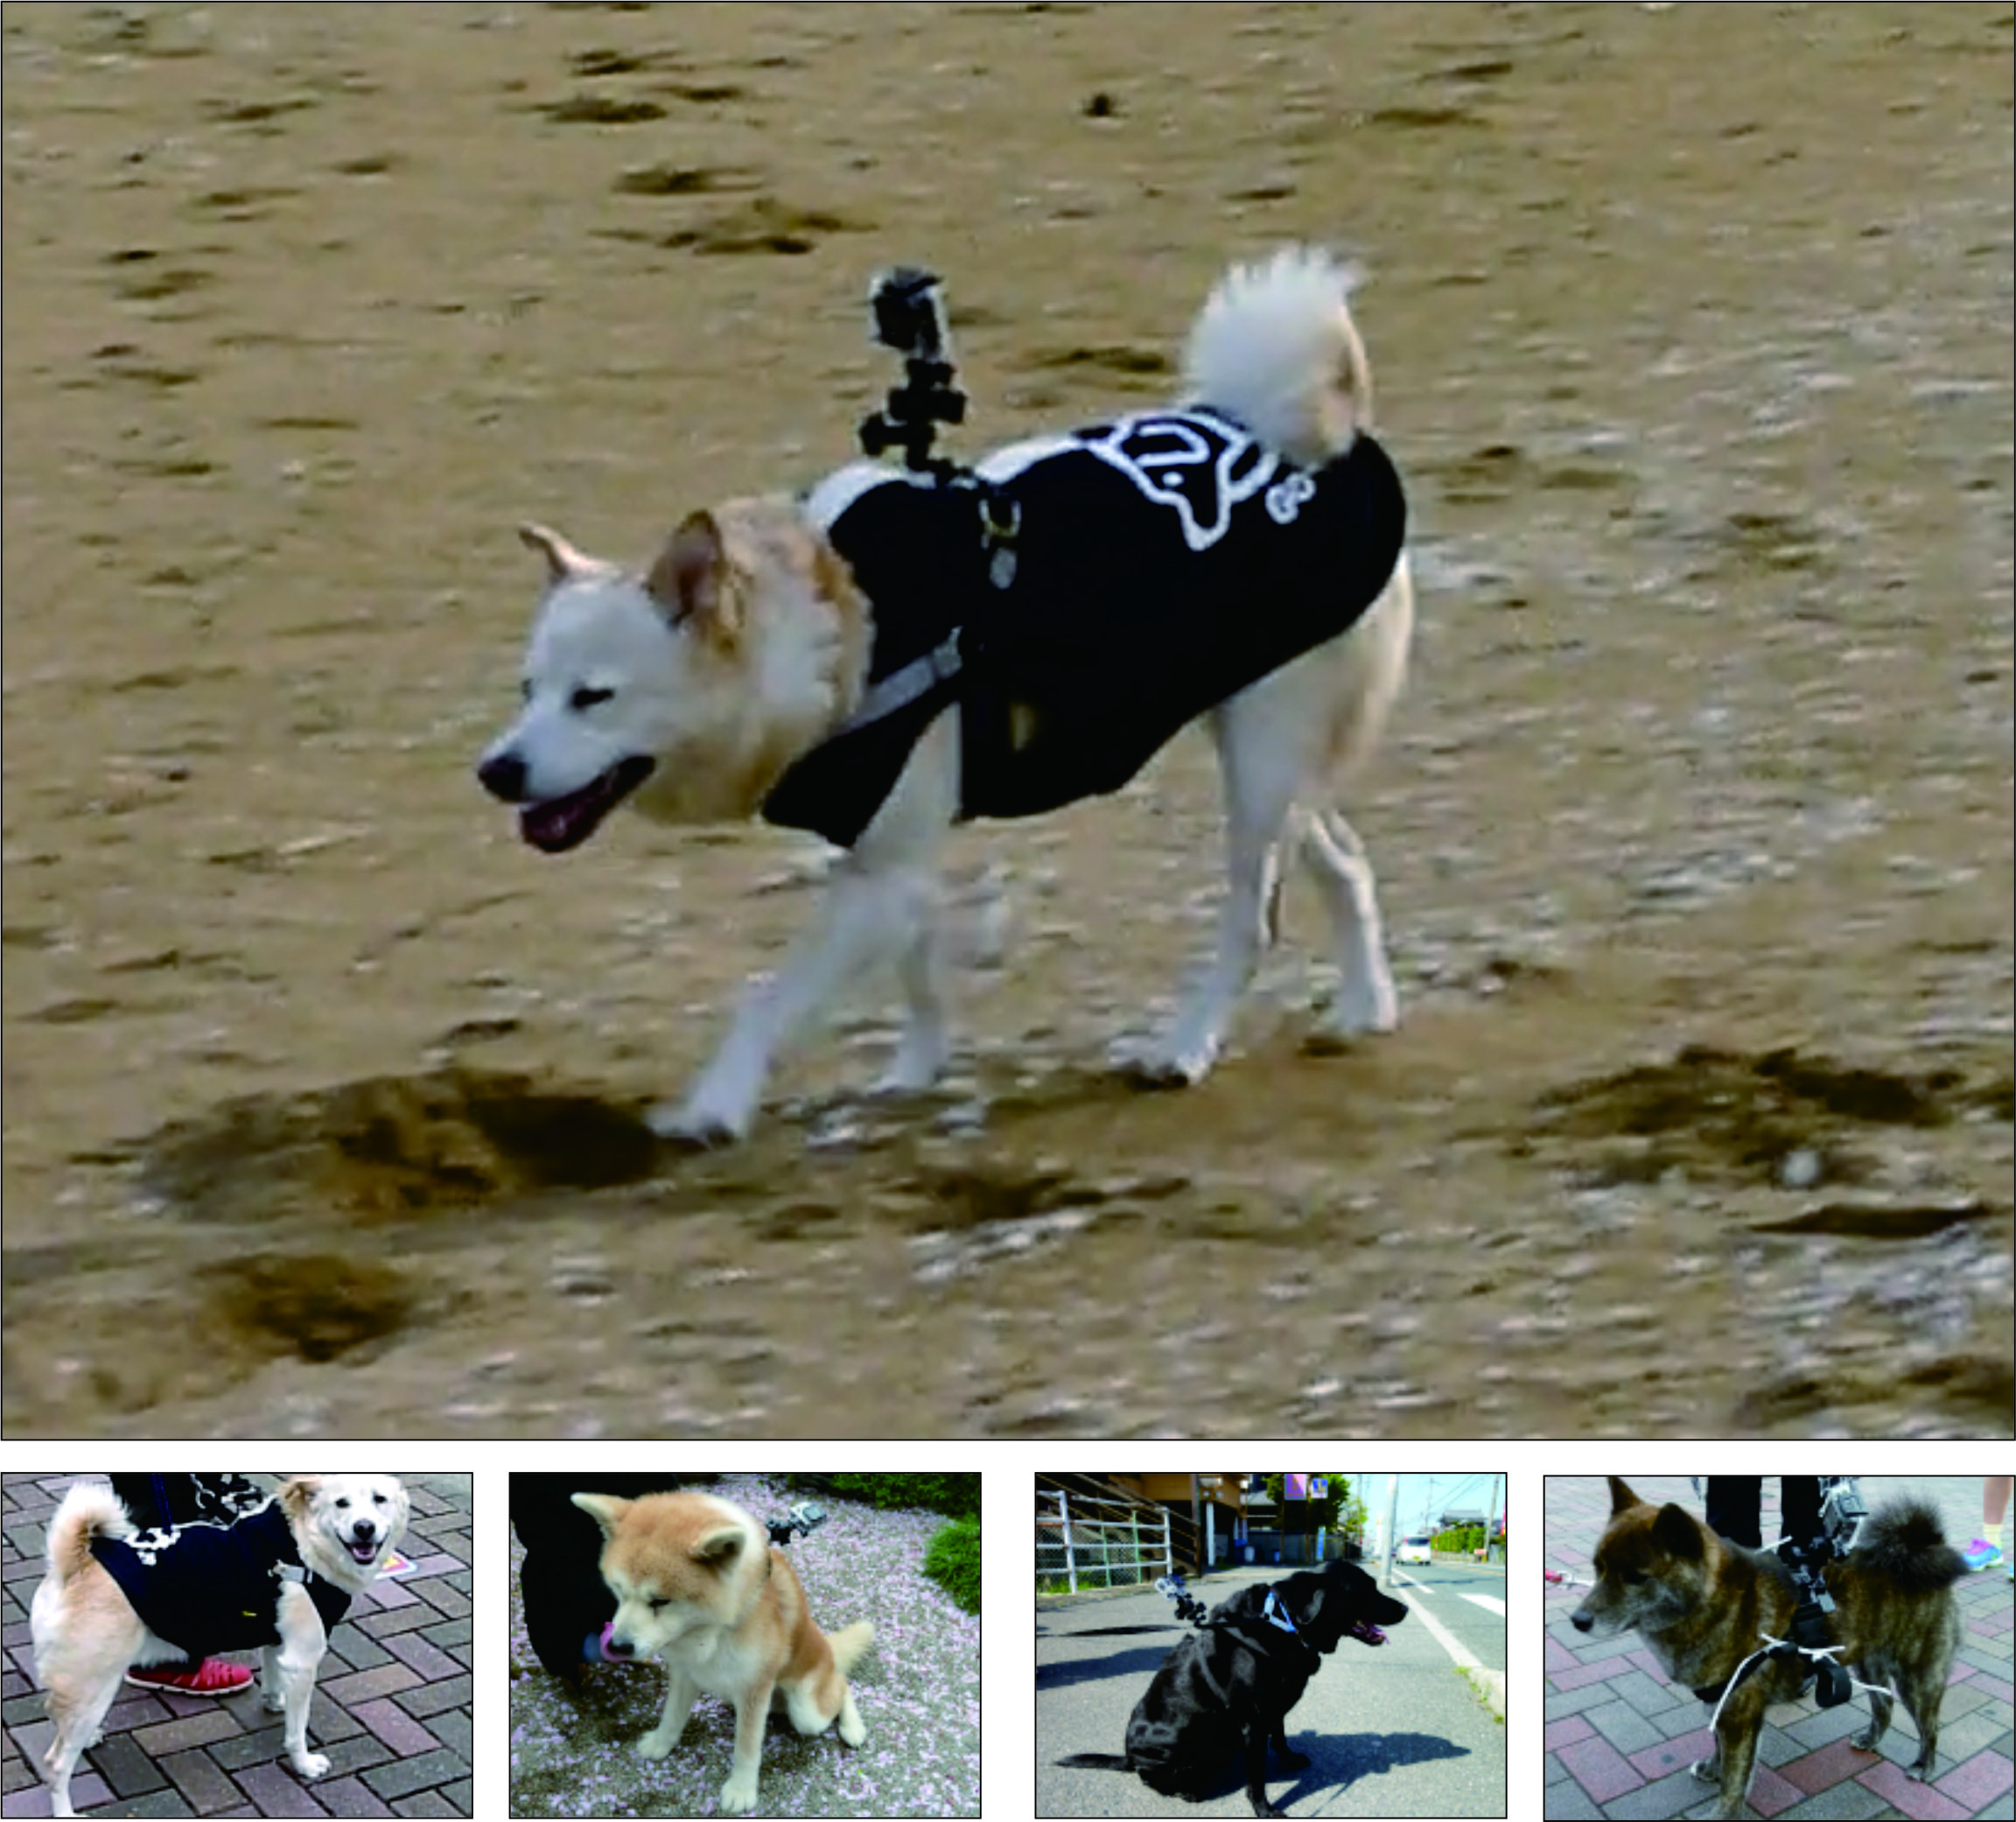
\includegraphics[width=0.8\textwidth]{figures/dogcentric}
	\caption{Egocentric cameras such as GoPro is typically mounted on the head of the dog in DogCentric dataset. This camera capture the action from first-person point of view. 
	} 
	\label{fig:dogcentric}
% 	\vspace{-4mm}
\end{figure}

A myriad of algorithms has been proposed  for action recognition in
videos, including local spatio-temporal  descriptors such as dense
trajectories \cite{wang2013dense}, \cite{wang2011action} and improved dense trajectories \cite{wang2013action}, and convolutional neural network
(CNN) based approach \cite{wang2015action}, \cite{simonyan2014two}, \cite{wang2015temporal}. However, those methods are not specifically
devised for  the first-person videos and thus in general can not provide
satisfactory detection performance in this scenario. Recently, some
approaches were suggested for the first-person action recognition. For
instance, Iwashita \textit{et al.} \cite{iwashita2014first} used the
conventional local and global motion descriptors and clustered them
into visual words. Ma \textit{et al.} \cite{ma2016going} addressed a
two-steam ConvNet architecture which incorporated both spatial and
temporal networks. However, it only considered the temporal
characteristics of videos and demanded a large number of training
samples. Ryoo \textit{et al.} \cite{ryoo2015pooled} tracked the
changes of the descriptor values by pooled time series. It,
however, only considered simple pooling strategies and some
important temporal information may be lost. Recently
Kahani \textit{et al.} \cite{kahani2016time} grouped the time series
feature and computed the linear correlation among these groups.
However, it requires a judicious  selection of the local time
windows.

In light of the non-stationary nature of the feature vectors, in
this \blue{thesis}, we, inspired by the success of Hilbert-Huang transform
(HHT) \cite{huang1998empirical} in EEG, ECG, %MEG
and other non-stationary signal analyses \cite{xie2006mean},
\cite{echeverria2001application}, consider a new method which aggregates
both of the short- and long-term trends based on the coefficients of
HHT. To achieve this, we apply HHT to the trajectory-pooled
deep-convolutional descriptors (TDD) \cite{wang2015action},
which includes both of the trajectory information
\cite{wang2013action}
and the deep-learned features \cite{simonyan2014two}, and treats the temporal dimension as feature channel.
HHT decomposes the TDD feature vector in each channel via a set of intrinsic mode
functions (IMFs) based on the empirical mode decomposition (EMD) and
then analyze the coefficients using Hilbert transform. Thereafter,
some  characteristics of the coefficients \cite{riaz2016emd} are
determined to render more precise feature representation.


To the authors' best knowledge, it is the first time HHT is employed
for action recognition in videos. This new approach possesses
several salient features. First, it can prune out noisy feature
channel by selecting an appropriate IMF combination through EMD.
Second, it can take both of the short- and long-term trends of the
video into consideration to render better understandings of
the trends or patterns of the features in the first-person videos.
The proposed approach can also be successfully incorporated with the
CNN features such as trajectory pooled CNN features to
achieve superior detection accuracy. Simulations show that
the proposed method outperforms the main state-of-the-art works on
two widespread public first-person datasets.



\begin{figure}[!t]
\centering
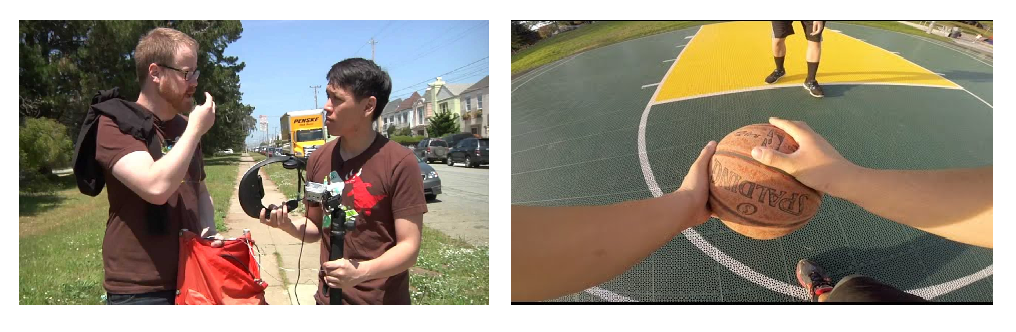
\includegraphics[width=0.85\textwidth]{figures/1s}
\caption{Differences in viewpoint in the first person to third person video videos. The left figure is the characteristic of the third person video, while the right figure is the characteristic of the first-person video.
} 
\label{fig:different}
%\vspace{-4mm}
\end{figure}


\section{Scope of this thesis}

\subsection{Problem Statements and Challenge}
\label{sec:problem-statements}
\blue{We focus on action recognition in the first-person/egocentric videos. The main challenge in this work are camera motion and wild motion caused by wearer's natural head motion which make video so shaky that hard to be analyzed. Also, the background also moving in the first-person video make the system hard to separating between foreground and background.}

\blue{Usually by determining the foreground object first, we can make our best representation descriptor. But, since the characteristic of the first-person video that background also moving, sometimes make the background be  important component to be extracted as foreground. }
	
\blue{We observe that in any egocentric video involving sub-action that move in the same time. We found that saliency image can benefit the system to make best feature descriptor. By extracting optical flow from two consecutive images, then applying some thresholds to obtain new saliency motion map representation, we can detect the fine-grained object and select the feature around it. We assume that the features extracted from fine-grained object is more important than the feature extracted from sub-objects.
We also focus on short-time term actions that typically last few seconds, e.g., pour, take, open etc. 
Fig. \ref{fig:kitchen} gives some examples of the actions we are interested in recognizing.}

\begin{figure}[!t]
	\centering
	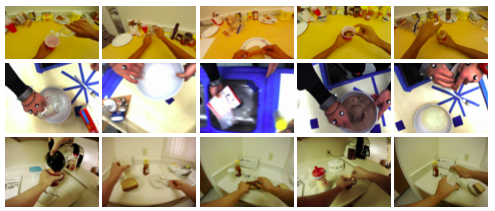
\includegraphics[width=0.95\textwidth]{figures/kitchen}
	\label{fig:kitchen}
	\caption{The action which we aim to recognize.
	} 
	%\vspace{-4mm}
\end{figure}

\blue{We also observe that frame selection is important task to increase the detection performance. Given a video, which consist of a lot of similar consecutive frames. Those similar consecutive images will produce the duplication of the descriptor, which influence the quality of the feature representation. Hence, the scheme need to be developed to circumvent this situations. 
We observe to do frame selection as preprocessing step. Given a video consists bunch of images, we pool them into sequel of time window. Then, we identify the most essential frame by performing pooling on the SVM.}

\blue{Convolutional neural network ($CNN$) which popular nowadays in many area can be useful tool for computer vision task. However, it produce a huge number of descriptor. We show that simple pooling strategy is not enough to deal with this, hence we employed non-stationary tool analysis, Hilbert-Huang Transform to aggregates the descriptor into one representative feature video.}

\blue{Furthermore, the datasets that we use in this work are very challenging. The characteristic of these three datasets are different each other. The first dataset, DogCentric dataset \cite{yumi2014first} is the most difficult one since the video recorded in dog head. This dataset is the shakiest dataset that we used in this thesis. The second dataset is JPL dataset \cite{ryoo2013first}, which use a doll as a model. The typical of this dataset is the interaction dataset. People will interact with the model in some action like hug, wave, punch, etc. While the last dataset \cite{spriggs2009temporal} is continues dataset which recorded in long period of time. Unbalanced number of video and the rough label annotation make the action classification even more harder.}


\subsection{Contributions}
\label{sec:contributions}
\blue{We propose a temporal aggregation for first-person video using non-stationary tools, Hilbert-Huang Transform. To the best author's knowledge, it the first time non-stationary tools used for temporal aggregation in computer vision area. We also perform background-foreground separation by selecting only the inlier trajectory. Also, the frame selection in the first part has increased the performance of detection. We have explored the generalization of our proposed method by performing in three different characteristics first-person point of view video. We show later that our technique can corporate with $CNN$ features and improve it performance. 
This work proposes a general temporal aggregation for first-person action recognition with following specific contributions:
}
\blue{
\begin{enumerate}
	\item We propose new temporal aggregation technique for first-person video by using Hilbert-Huang transform (HHT). To the best of author's knowledges, this is the first-time that HHT employed for action recognition in video.
	\item We propose dominant motion saliency object and its trajectory to select inlier trajectories to prune the noisy features caused by camera moving in first-person video.
	\item Our feature representation can prune out noisy feature
	channel by selecting an appropriate IMF combination through EMD. Also, Our feature can take both of the short- and long-term trends of the
	video into consideration to render better understandings of
	the trends or patterns of the features in the first-person videos.
	\item We propose frame selection in the preprocessing part to improve the detection performance.
    
\end{enumerate}
}
\section{Thesis Outline}
\blue{Brief outline of text in this thesis is as follows. In chapter 2, we review of the related work. In chapter 3, we explain our contributions on the proposed approaches for first-person action recognition which is temporal aggregation using Hilbert-Huang transform. In chapter 4, we explain our experimental and result. 
Finally, we end the thesis with concluding remarks and future work.} 



	
\chapter{Related Work}
A myriad of algorithms have been proposed  for action recognition in
videos, including local spatio-temporal  descriptors such as dense
trajectories \cite{wang2013dense, wang2011action} and improved dense
trajectories \cite{wang2013action}, and convolutional neural network
(CNN) based approach \cite{wang2015action, simonyan2014two,
wang2015temporal}. However, those methods does not specifically
devised for first-person videos and thus in general can not provide
satisfactory detection performance in this scenario. 

Recently, some
approaches were suggested for first-person action recognition. For
instance,
Iwashita \textit{et al.} \cite{iwashita2014first} used the
conventional local and global motion descriptors and clustered them
into visual words. Ma \textit{et al.} \cite{ma2016going} addressed a
two-steam ConvNet architecture which incorporated both spatial and
temporal networks. However, it only considered the temporal
characteristics of videos and demands a large number of training
samples. Ryoo \textit{et al.} \cite{ryoo2015pooled} tracked the
changes of the descriptor values by pooled time series. It,
however, only considered simple pooling strategies and some 
important temporal information may be lost. Recently
Kahani \textit{et al.} \cite{kahani2016time} grouped the time series
feature and computed the linear correlation among these groups.
However, it requires a judicious  selection of the local time
windows.

Camera motion is the main characteristic of first-person video, which very common in real-world. It be a main challenge of action recognition in first-person video algorithm. \cite{kraft2014motion, jain2013better} propose method to decompose visual motion and extracting the trajectories and make descriptor. 


	
	\newpage
\chapter{Proposed Method}
\section{Deep Learned Features for Action Recognition in First-Person Video}

asd 
\begin{figure}[htttp]
\centering
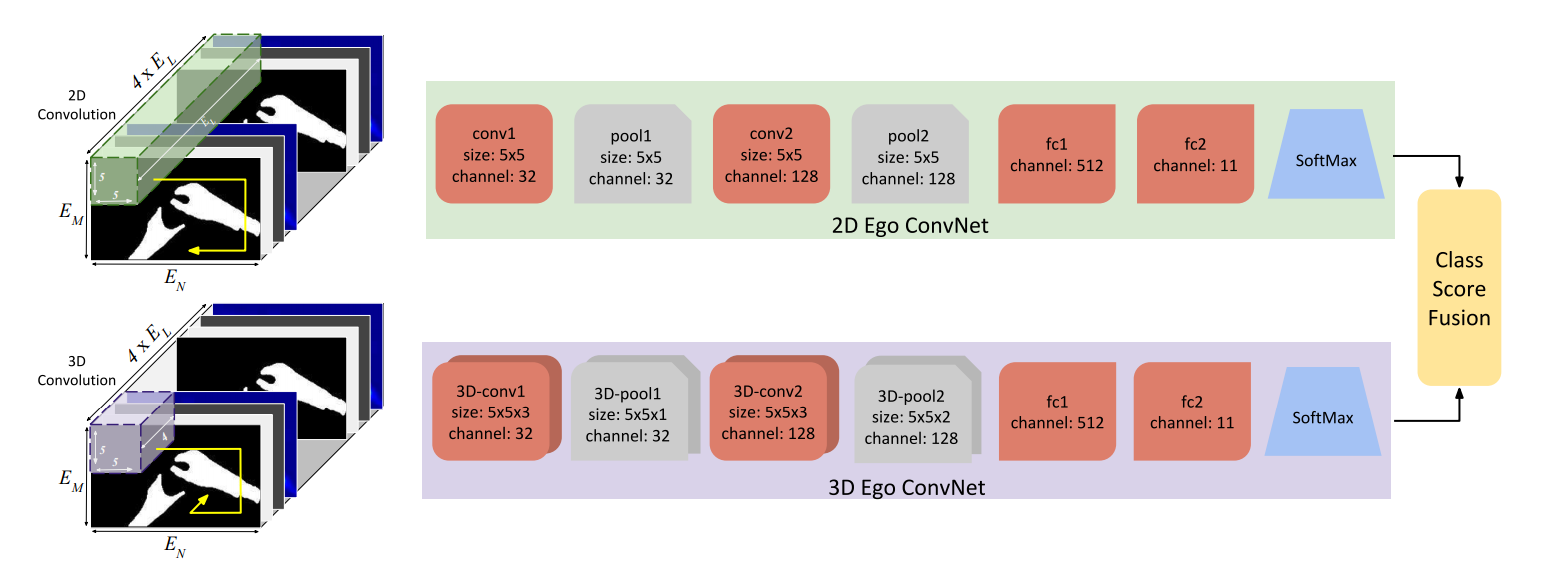
\includegraphics[width=1\textwidth]{figures/framework2}
\caption{Overview of the proposed action recognition scheme for the first-person video.
} 
\label{fig:framework}
%\vspace{-4mm}
\end{figure}

\section{Temporal Aggregation Using Hilbert-Huang Transform }

In this section, we introduce the proposed  HHT-based temporal
aggregation  method for first-person videos. The new method begins
with feature extraction using CNN \cite{wang2015action} and then
invokes HHT on the features by first decomposing the features with
EMD and conducting time-frequency analysis with Hilbert transform
for each IMF decomposed features. Finally, we analyze the
statistical properties of some desirable features to construct our
feature representation. For easy reference, the overall procedures
of the proposed method are as illustrated in Fig.
\ref{fig:framework}.

\subsection{Trajectory-pooled Deep-convolutional Descriptors}
In this section, we briefly review the TDD feature extraction
\cite{wang2015action}. % We  first use the trajectory-pooled
%deep-convolutional descriptors.
The deep-learned based features takes advantage of the image
appearance and motion information as descriptors.
%. This deep-learned
It first uses the ConvNets architecture and is trained on large
datasets in order to extract multi-scale convolutional maps. Then,
TDD employs the improved trajectories to aggregate an efficient
feature representation by sampling and pooling. We also apply both
spatio-temporal and channel normalization to the TDD features to
boost the performance. Finally, we combine those features to
obtain a TDD feature vector.

\begin{figure}[!t]
\centering
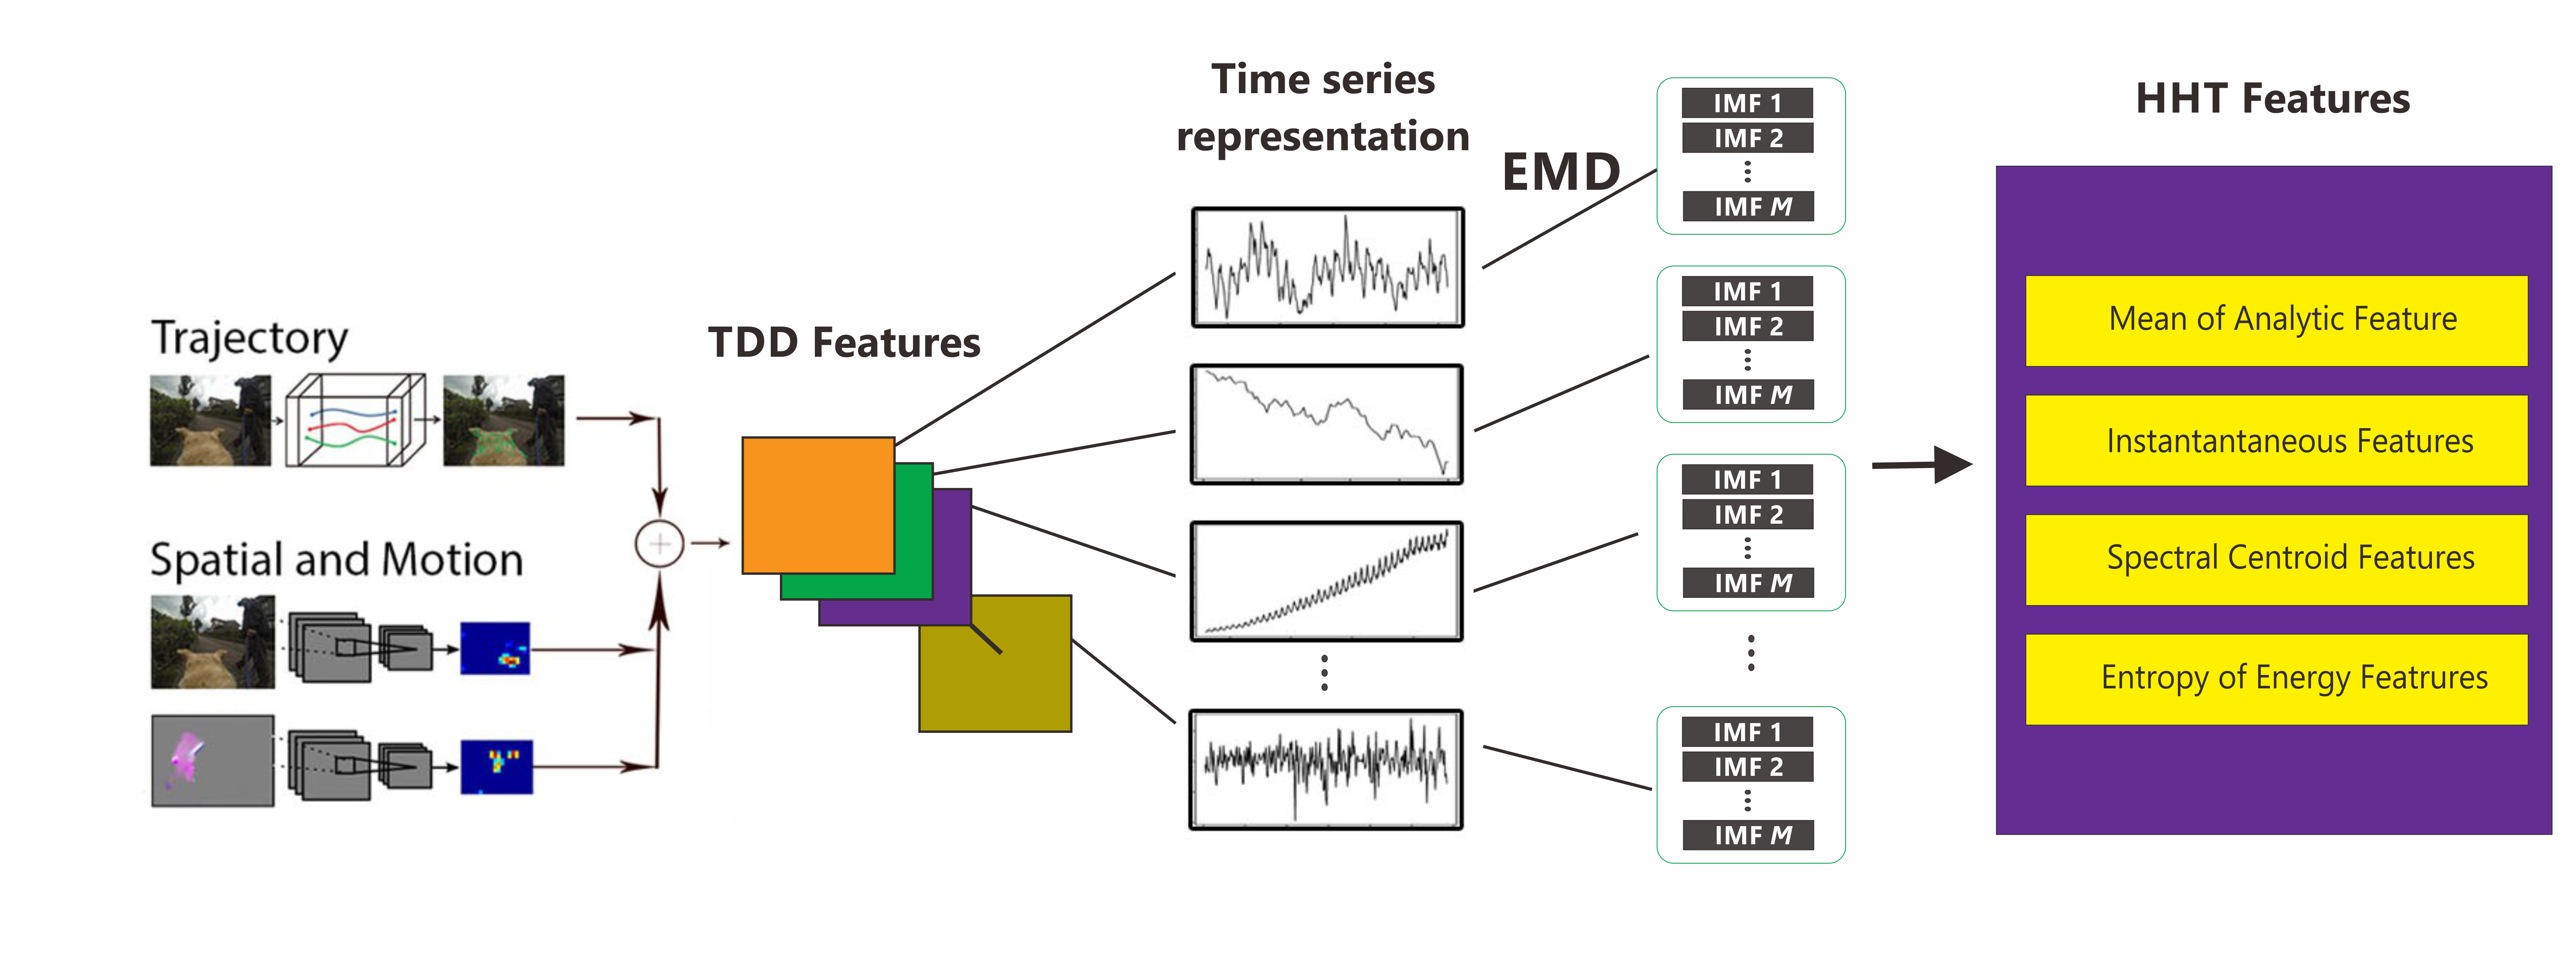
\includegraphics[width=1\textwidth]{figures/framework}
\caption{Overview of the proposed action recognition scheme for the first-person video.
} 
\label{fig:framework}
%\vspace{-4mm}
\end{figure}

\subsection{Empirical Mode Decomposition}

After determining the TDD descriptors in feature extraction,
this subsection describes EMD, a way to decompose signals into a
number of IMFs. Given a feature descriptor, which is in general
non-stationary, with dimension  $k \times l$, where $k$ and $l$ are
the numbers of the spatio-temporal features and  feature channel,
respectively, we apply EMD to the descriptor in each feature channel
to obtain a set of IMFs by the following steps, where for simplicity
the feature is denoted as $x(n)$.
\begin{enumerate}
    \item Identify both maxima and minima (extremes) of  $x(n)$.
    \item Interpolate between minima and maxima to generate the envelopes  $e_{l}(n)$ and $e_{m}(n)$.
    \item Calculate the local mean by  $a(n)=(e_{m}(n)+e_{n}(n))/2$.
    \item Extract the detail  $h_{1}(n) = x(n) - a(n)$.
    \item Decide whether $h_{1}(n)$ is IMF or not. If the number of extremes and zero crossing of  $h_{1}(n)$ are the same or differ by at most one and at any point the average value of the envelope defined by both local maxima and minima are zero, then  $h_{1}(n)$  is regarded as IMF; otherwise, it is not.
    \item Repeat steps 1 to 5 until we get all of IMFs.
\end{enumerate}

Finally, $x(n)$ can be represented as
\begin{equation}
      x(n) = \sum_{m=1}^{M} c_{m}(n) + r_{M}(n)
\end{equation}
where $M$ denotes the number of IMFs, $c_{m}(n)$ is the $m$th IMF of
the feature  $x(n)$ and $r_{M}(n)$ stands for the residue.

\subsection{Hilbert Transform Analysis}
Based on the IMFs determined above, this subsection
describes the Hilbert transform analysis  to extract the desired
features. For this, we conduct the Hilbert transform with
respect to IMFs and obtain
analytic signals %which will be used as our first feature.
%%Denote IMF as $c_{m}(t)$,
%we  determine our analytic signals by the Hilbert transform
%given by




\begin{equation}
{\cal H}[c_{m}(n)] = \frac{1}{\pi}\sum_{n' = 1 }^{K
}\frac{c_{m}(n')}{n-n'}
\end{equation}
where $K$ is the length of $c_{m}(n)$. The associated analytic
signal can then be expressed as


\begin{equation}
    z_{m}(n) = c_{m}(n) + jH[c_{m}(n)] = a_{m}(n)e^{j\phi_{m}(n)}
\end{equation}

%Based on {\blue $z_{m}(n)$},
Next, we consider four features associated with the
%statistical
characteristics of $z_{m}(n)$, {\it i.e.} mean,
instantaneous frequency, spectral centroid \cite{riaz2016emd}, and
entropy of energy \cite{tolwinski2007hilbert}. The  mean feature of
$z_{m}(n)$  is given by
\begin{equation}
    \mu_{m}(n) = \frac{1}{K}\sum_{n=1}^{K} z_{m}(n)
\end{equation}


The instantaneous frequency feature %of each IMF
is given by
\begin{equation}
f_{m}(n) = \frac{1}{4\pi}(\phi_{m}(n+1)-\phi_{m}(n-1))
\end{equation}

%Apart from instantaneous frequency, we also  take the spectral centroid information \cite{riaz2016emd} as our third feature {\blue by
The spectral centroid feature,  $C_{s}^{m} $, is given by
\begin{equation}
    C_{s}^{m} = \frac{\sum_{f_{m}}2 \pi f_{m}P(f_{m})}{\sum_{f_{m}}P(f_{m})}
\end{equation}
where $P(w)$ is power spectral density of  $z_{m}(n)$
\cite{riaz2016emd}.

The log of entropy feature is given by
\begin{equation}
    H_{m} = - \sum_{i=1}^{N}p_{i} \ \textup{log} \ p_{i}
\end{equation}
where $p_{i}$ is the probability of energy level $E_{i}
=log(\sum_{n=1}^{K}|z_{m}(n)|^{2})$ appears.


Finally, we can use these four features individually or
combine them together into a single feature vector as our final
feature representation.

	
	\newpage
\chapter{Experimental and Result}
\label{sec:Experiment}
\section{Dataset}

In this section, we assess the performance of the proposed method as
compared with previous works through exhaustive computer simulations
based on three famous public first-person video datasets including
DogCentric \cite{yumi2014first}, JPL First-Person Interaction
\cite{ryoo2013first}, and Kitchen \cite{spriggs2009temporal} which contain a variety of action
taken from model's view point. The example images from these datasets are shown in Appendix \ref{appendix_a}.


\begin{table}[!b]
    \centering
    \begin{tabular}{c|c|c|c|c}
        \hline
        \hline
        Dataset &  Subject & Videos & Class & Baseline Accuracy\\
        \hline
        DogCentric & 4 & 205 & 10 & 74.56\% \\
        JPL dataset & 4 & 205 & 10 & 74.56\% \\
        \hline
    \end{tabular}
    \caption{Survey of the dataset and the banchmark method accuracy.}
    \label{tab:my_label}
\end{table}


\subsection{Evaluation Protocol Experiment Setup}


To evaluate our work, we mainly follow the suggestions provided by
the first-person video datasets. For Dogcentric dataset
\cite{yumi2014first}, %following standard evaluation setting,
we randomly select half of video sequences of each activity from our
dataset as the training data and use the rest of the sequences for
testing 100 times and average the results.  The Dogcentric dataset
consists of 10 class activities: Ball play, Car, Drink, Feed, Turn
left, Turn right, Pet, Body shake, Sniff, and Walk. As for the JPL
First-Person Interaction dataset \cite{ryoo2013first}, which consist
of 7 class activities: Hand shake, Hug, Pet, Wave, Point-Converse,
Punch, and Throw, the protocols are the same as the Dogcentric
dataset.

As the feature descriptors, we use the features extracted by TDD
with spatial information from convolutional layer 5 and temporal
information from convolutional layer 4. %, as these features in general
%provide better performance according to our experience.
Also, we only use the first 10,000 samples in each feature channel
to conduct EMD  to reduce the dimension of the feature vectors. We
used SVM classifier with $c=100$ and linear kernel in all of our
experiments. Also, $L_{2}$ normalization is applied to each feature
vector.
	\newpage
\chapter{Conclusion and Future Directions}
This paper has developed an efficacious HHT-based temporal
aggregation method for first-person action recognition, which takes
account of the non-stationary characteristics of the feature
vectors. Through EMD in HHT, the proposed method can aggregate both
of the short- and long-term trends based on the coefficients of HHT.
The new method can be employed with TDD features to achieve superior
detection performance. Conducted experiments show that the proposed
method outperforms the main state-of-the-art methods  on two popular
DogCentric and JPL datasets.
	%\input{sections/References.bib}
%----------------------------------------------------------------------------------------------------------------------------------------------------------
	% back pages 後頁
	%
% this file is encoded in utf-8
% v1.7

%%% 參考文獻
\newpage
\chapter*{\textit{Appendix} A} 
\label{appendix_a}
\addcontentsline{toc}{chapter}{\textit{Appendix A}: Example images from the datasets}
\renewcommand{\bibname}{\protect\makebox[5cm][s]{Appendix}}
\label{appendix_a}
\textbf{Example images from the datasets}

\begin{figure}[http]
\centering
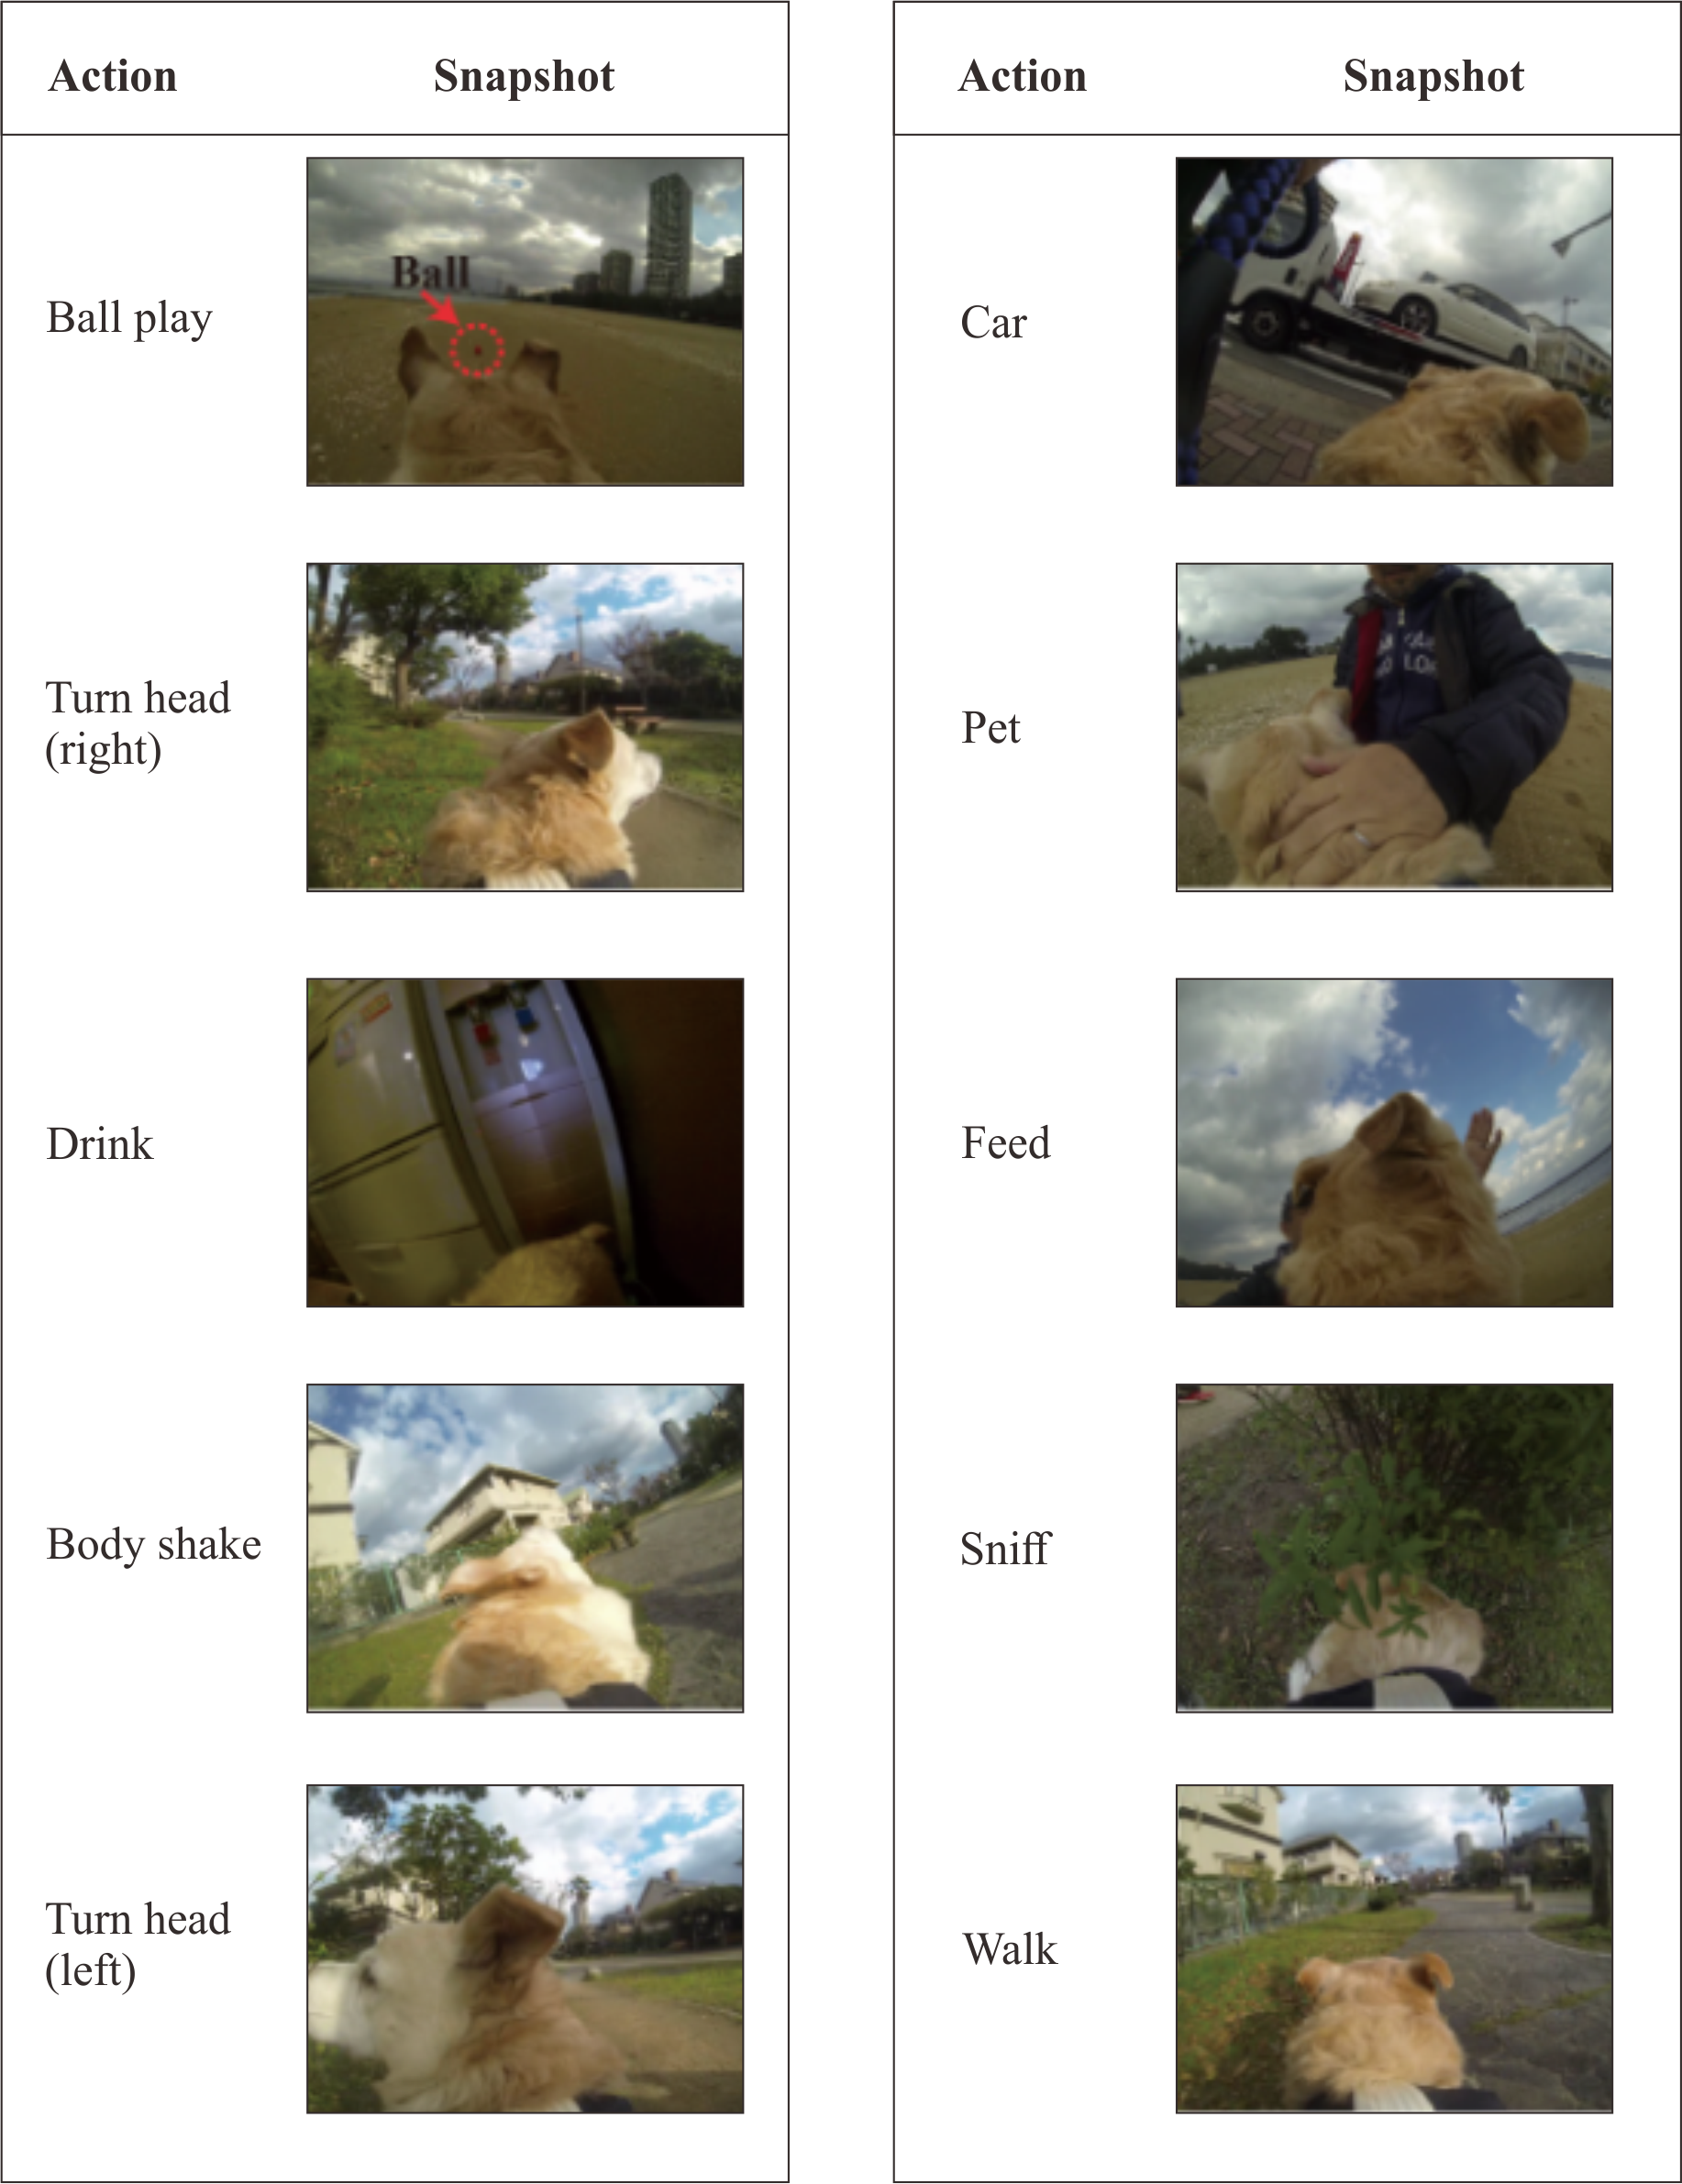
\includegraphics[width=0.8\textwidth]{figures/appendix_a}
\caption{Snapshot of the DogCentric dataset} 
\label{fig:append1}
%\vspace{-4mm}
\end{figure}

\begin{figure}[!t]
\centering
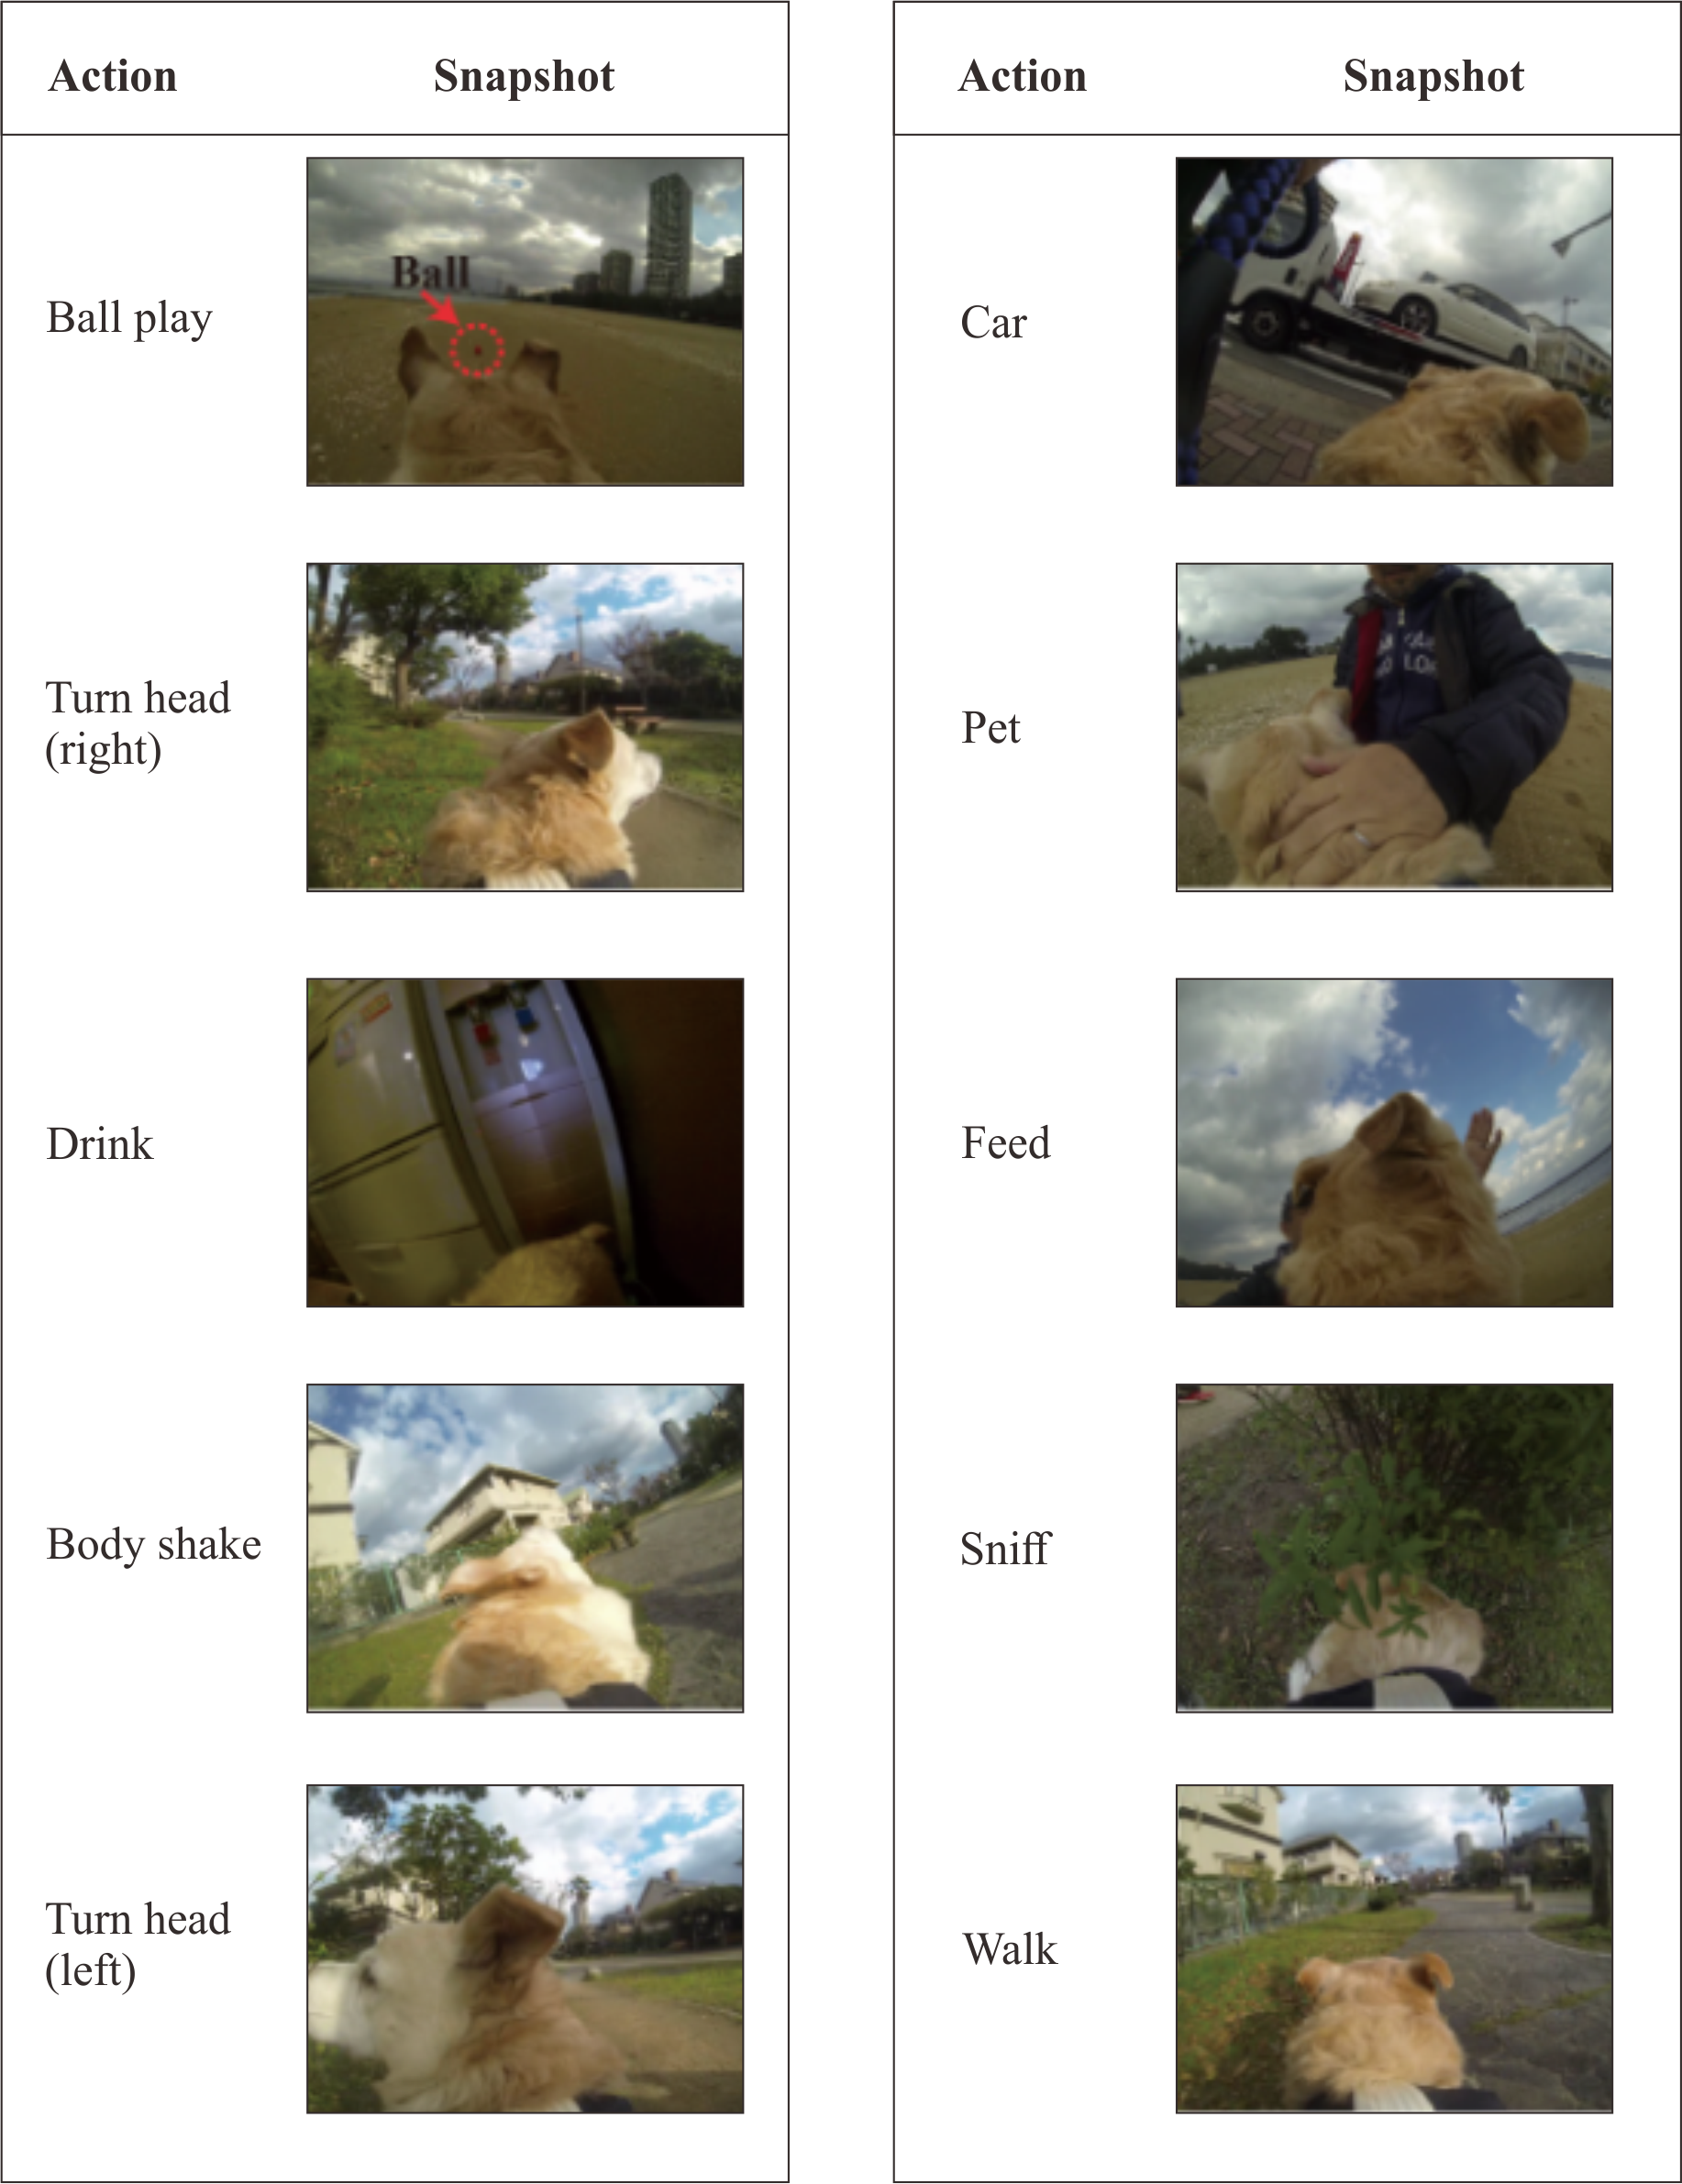
\includegraphics[width=0.8\textwidth]{figures/appendix_a}
\caption{Snapshot of the JPL dataset} 
\label{fig:append2}
%\vspace{-4mm}
\end{figure}

\begin{figure}[!t]
\centering
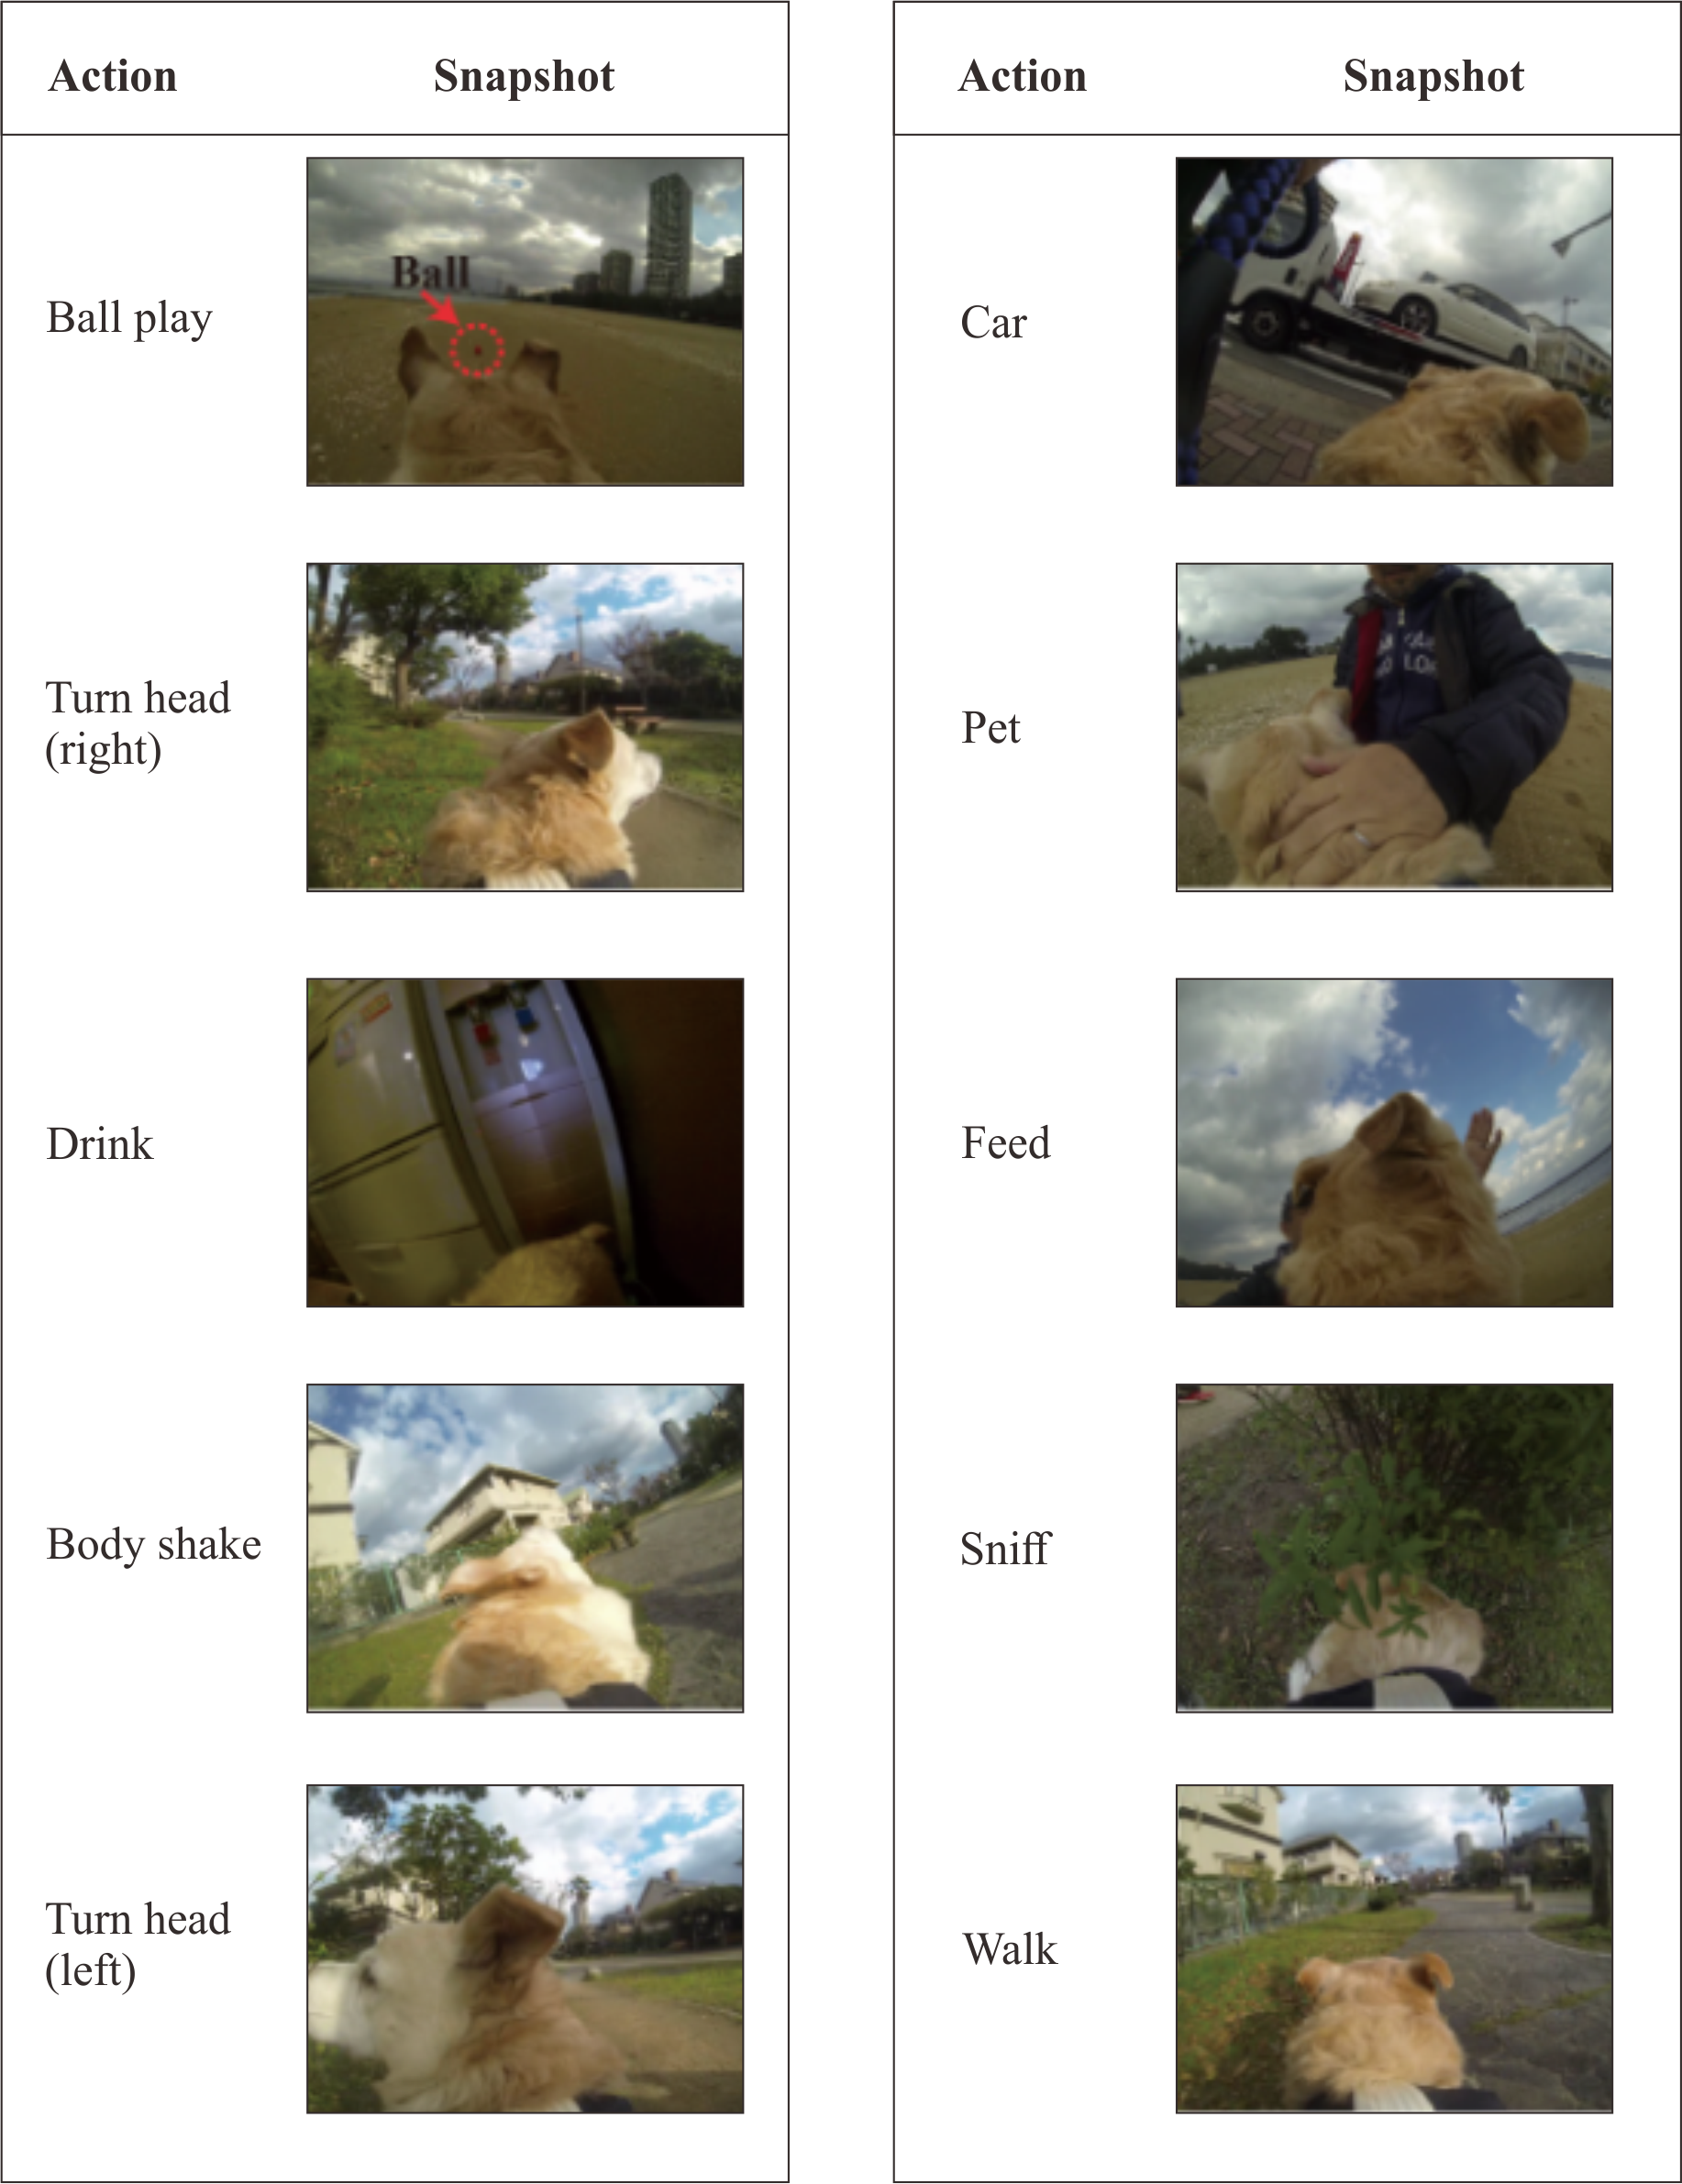
\includegraphics[width=0.8\textwidth]{figures/appendix_a}
\caption{Snapshot of the Kitchen dataset} 
\label{fig:append3}
%\vspace{-4mm}
\end{figure}



\newpage
\addcontentsline{toc}{chapter}{\nameRef}
\renewcommand{\bibname}{\protect\makebox[5cm][s]{\nameRef}}
%  \makebox{} is fragile; need protect
%\bibliographystyle{alpha}  % 使用 IEEE Trans 期刊格式
\bibliographystyle{ieeetr}  % 使用 IEEE Trans 期刊格式
\bibliography{my_bib}  %reference 所需的bib檔
%\bibliography{my_bib}  %reference 所需的bib檔

%%% 附錄



\end{CJK}  %%% ZZZ %%%
\end{document} 
 